\documentclass[11pt,a4paper,spanish]{book}
\usepackage{estilo_unir-1}
\usepackage{apacite}

\usepackage{hyperref}
\usepackage{longtable}
\numberwithin{equation}{chapter}
%\usepackage{caption}
\numberwithin{figure}{chapter}
%\usepackage{chngcntr}
%\counterwithin{equation}{chapter}
%\counterwithin{figure}{chapter}
%\counterwithin{table}{chapter}
%\renewcommand\theequation{\thechapter.\arabic{equation}}
%\renewcommand\thefigure{\thechapter.\arabic{figure}}
%\renewcommand\thetable{\thechapter.\arabic{table}}
%\renewcommand\theequation{\thechapter.\arabic{equation}}
%\counterwithin{figure}{chapter}
%\counterwithin{table}{chapter}
%\renewcommand\thefigure{\thechapter.\arabic{figure}}
%\renewcommand\thetable{\thechapter.\arabic{table}}
%\renewcommand\thefigure{\thechapter.\arabic{figure}}
%\makeatletter
%\renewcommand\p@figure{\thechapter..\arabic{figure}}
%\makeatother



%---------------------------
%título del trabajo y autor
%---------------------------
\title{Desarrollo de un Sistema Híbrido de Asistencia Clínica: Fine-Tuning de LLMs Open Source y Arquitectura RAG (Retrieval-Augmented Generation) para Medicina Basada en la Evidencia.}
\titulacion{Máster en Inteligencia Artificial}
\author{David Solanas Sanz}
\date{1 de junio de 2026}
\director{Andrés Soto Villaverde}
\nombreciudad{Zaragoza}

%---------------------------
%marges
%---------------------------
%\usepackage[margin=1.9cm]{geometry}
%---------------------------
%---------------------------
%---------------------------
%---------------------------
\setlength{\headheight}{26pt}
\addtolength{\topmargin}{-12pt}

\begin{document}
\renewcommand{\listfigurename}{Índice de Ilustraciones}
\renewcommand{\listtablename}{Índice de Tablas}
\renewcommand{\contentsname}{Índice de Contenidos}
\renewcommand{\figurename}{Figura}
\renewcommand{\tablename}{Tabla} 

\maketitle

\frontmatter
\tableofcontents
\listoffigures
\listoftables

\chapter{Resumen}
{\bf Nota:} En este apartado se introducirá un breve resumen en español del trabajo realizado (extensión máxima: 150 palabras). Este resumen debe incluir el objetivo o propósito de la investigación, la metodología, los resultados y las conclusiones.


{\bf Palabras Clave:} Se deben incluir de 3 a 5 palabras claves en español

\chapter{Abstract}
{\bf Nota:} En este apartado se introducirá un breve resumen en español del trabajo realizado (extensión máxima: 150 palabras). Este resumen debe incluir el objetivo o propósito de la investigación, la metodología, los resultados y las conclusiones.


{\bf Palabras Clave:} Se deben incluir de 3 a 5 palabras claves en inglés




\mainmatter
\chapter{Introducción}

%El primer capítulo es siempre una introducción. En la introducción se debe resumir de forma esquemática pero suficientemente clara lo esencial de cada una de las partes del trabajo. La lectura de este primer capítulo ha de dar una idea clara de lo que se pretendía, las conclusiones a las que se ha llegado y del procedimiento seguido.
%
%Como tal, es uno de los capítulos más importantes de la memoria. Las ideas principales a transmitir son la identificación del problema a tratar, la justificación de su importancia, los objetivos generales a grandes rasgos y un adelanto de la contribución que esperas hacer.
%
%Típicamente una introducción tiene tres apartados:
%\begin{itemize}
%\item Motivación / justificación del tema a tratar
%\item Planteamiento del trabajo
%\item Estructura del trabajo
%\end{itemize}


\section{Motivación y justificación}
La medicina actual se enfrenta al siguiente problema: el mismo crecimiento del conocimiento científico que debería mejorar la atención al paciente amenaza con desbordar la capacidad cognitiva del profesional clínico que ha de asimilarlo. \cite{rebitzer_influence_2008} identificaron este fenómeno como una forma específica de sobrecarga de información en el ámbito sanitario, argumentando que el volumen y la velocidad de publicación de nueva evidencia supera la capacidad individual de procesamiento de los médicos. Las consecuencias son las siguientes: adopción lenta de nuevos tratamientos, mayor probabilidad de pasar por alto hallazgos relevantes y, en última instancia, una reducción de la calidad asistencial. \cite{laker_quality_2018} profundizaron en esta problemática, demostrando que la sobrecarga informacional no solo afecta a la velocidad de la toma de decisiones clínicas, sino también a su calidad, introduciendo sesgos sistemáticos porque el médico prioriza solo los datos que han sido resaltados, ignorando otros hechos que podrían ser igual de importantes.

Ante esta situación, los Grandes Modelos de Lenguaje (LLM, por sus siglas en inglés) han emergido como una tecnología con potencial para actuar como interfaz inteligente entre el profesional clínico y el corpus de literatura científica disponible. Modelos como GPT-4 \cite{openai_gpt-4_2024} y LLaMA \cite{grattafiori2024llama3herdmodels} han demostrado capacidades notables de comprensión y generación de lenguaje natural, y revisiones sistemáticas recientes ya destacan su utilidad en tareas clínicas como asistencia al diagnóstico, triaje o soporte documental quirúrgico \cite{jcm13113041}. Sin embargo, su aplicación directa en entornos clínicos presenta limitaciones críticas que impiden su adopción directa sin mediación técnica adicional. La más relevante es la tendencia de estos modelos a generar información plausible pero factualmente incorrecta, fenómeno conocido en la literatura como alucinación \cite{ji_survey_2023}. En el dominio sanitario, donde una respuesta incorrecta puede tener consecuencias directas sobre decisiones terapéuticas, esta limitación es inaceptable. \cite{pal_med-halt_2023} cuantificaron este riesgo específicamente en contextos médicos, evidenciando tasas de error significativas incluso en modelos de última generación cuando operan fuera de su distribución de entrenamiento.

Para mitigar estas limitaciones, la arquitectura Retrieval-Augmented Generation (RAG) propuesta por \cite{lewis_retrieval-augmented_2021} ofrece un marco técnico que combina la capacidad generativa de los LLM con la recuperación dinámica de información desde fuentes de conocimiento externas verificadas. En el dominio sanitario, \cite{amugongo_retrieval_2025} han revisado sistemáticamente la aplicación de RAG en entornos clínicos, concluyendo que la integración de bases de conocimiento biomédico estructuradas reduce la tasa de alucinaciones y mejora la trazabilidad de las respuestas generadas, y señalando además la ausencia de marcos de evaluación estandarizados como una de las principales debilidades de la literatura existente. Complementariamente, el ajuste fino (fine-tuning) de modelos base sobre corpus clínicos especializados, como los estudiados por \cite{lee_biobert_2020} y \cite{alsentzer_publicly_2019}, ha demostrado mejorar la coherencia terminológica y la adecuación del formato de respuesta al contexto sanitario. La evaluación sistemática del efecto diferencial de cada componente (RAG y fine-tuning) mediante un diseño ablativo de cuatro configuraciones, sobre métricas estandarizadas, es una práctica aún poco extendida en la literatura clínica revisada \cite{amugongo_retrieval_2025}.

Este trabajo se sitúa en la intersección de ambas líneas técnicas, proponiendo un sistema híbrido que combina el fine-tuning mediante QLoRA (\textit{Quantized Low-Rank Adaptation}) sobre datos clínicos con una arquitectura RAG conectada a PubMed, con el objetivo de construir un asistente de consulta bibliográfica para profesionales sanitarios que sea simultáneamente preciso, trazable y clínicamente coherente.

\section{Planteamiento del trabajo}
El objetivo principal de este Trabajo de Fin de Estudios es diseñar, implementar y evaluar un sistema híbrido de asistencia a la consulta bibliográfica clínica que combine fine-tuning eficiente de un LLM con una arquitectura RAG sobre literatura biomédica verificada, analizando la contribución diferencial de cada componente sobre la calidad de las respuestas generadas.

Los objetivos específicos que operacionalizan este propósito son los siguientes:
\begin{itemize}
	\item Construir un pipeline de ingestión, fragmentación e indexación semántica de artículos biomédicos de PubMed en una base de datos vectorial, empleando embeddings especializados en dominio clínico.
	\item Realizar el ajuste fino del modelo LLaMA-3.1-8B mediante QLoRA sobre el corpus de transcripciones clínicas MTSamples, adaptando el estilo y la terminología de las respuestas al contexto sanitario.
	\item Integrar ambos módulos en una arquitectura híbrida gestionada mediante prácticas MLOps (\textit{Machine Learning Operations}), garantizando la reproducibilidad y trazabilidad del ciclo experimental.
	\item Evaluar el sistema bajo cuatro configuraciones experimentales (modelo base, fine-tuning exclusivo, RAG exclusivo y sistema híbrido completo) con el fin de cuantificar la contribución individual de cada componente sobre métricas de calidad de recuperación y generación.
	\item Determinar si el sistema híbrido ofrece ventajas cuantificables sobre las configuraciones parciales, identificando qué limitación específica resuelve cada técnica.
\end{itemize}

La contribución diferencial de este trabajo respecto a los estudios previos no reside en la novedad del diseño ablativo en sí, ya empleado en otros dominios por \cite{balaguer2024ragvsfinetuningpipelines} y en pregunta-respuesta médica genérica por \cite{pingua_medical_FT_vs_RAG_2025}, sino en tres aspectos concretos. En primer lugar, en su aplicación al escenario específico de la asistencia bibliográfica clínica sobre literatura primaria de PubMed. En segundo lugar, en su realización íntegra sobre un único modelo de código abierto cuantizado en hardware modesto. Y en tercer lugar, en la incorporación de mecanismos explícitos de verificación automática de citaciones y abstención que permiten cuantificar de forma directa la contribución de RAG a la reducción de alucinaciones, complementando las métricas RAGAS estandarizadas \cite{es2025ragasautomatedevaluationretrieval}.

\section{Estructura del trabajo}
Este trabajo se organiza en siete capítulos, los cuales se organizan de la siguiente manera:

El \textbf{Capítulo 1 (Introducción)} presenta la problemática de la sobrecarga informacional en medicina, justifica la relevancia del trabajo y enuncia sus objetivos generales.

El \textbf{Capítulo 2 (Contexto y Estado del Arte)} revisa la literatura sobre los fundamentos técnicos del sistema: arquitecturas Transformer y LLMs, técnicas de ajuste fino eficiente (LoRA y QLoRA), la arquitectura RAG, los modelos de embeddings biomédicos, las bases de datos vectoriales y los marcos de evaluación. El capítulo concluye con una síntesis y brecha identificada en la literatura que justifica la contribución del trabajo.

El \textbf{Capítulo 3 (Objetivos y Metodología de Trabajo)} define los objetivos específicos del trabajo de forma SMART y describe la metodología seguida para alcanzarlos, incluyendo el diseño experimental ablativo de cuatro configuraciones, las herramientas empleadas y la planificación temporal.

El \textbf{Capítulo 4 (Identificación de Requisitos)} especifica los requisitos funcionales y no funcionales del sistema, el perfil de usuario objetivo y el proceso de validación de requisitos.

El \textbf{Capítulo 5 (Descripción de la Herramienta Software Desarrollada)} detalla la arquitectura del sistema, los módulos implementados (ingestión, embeddings, fine-tuning, pipeline RAG e interfaz Gradio) y las decisiones de diseño adoptadas.

El \textbf{Capítulo 6 (Evaluación)} presenta los resultados de la evaluación automática mediante RAGAS para las cuatro configuraciones experimentales, junto con un conjunto de métricas deterministas de comportamiento de citación, así como una evaluación heurística de usabilidad y aplicabilidad de la herramienta realizada por el autor.

El \textbf{Capítulo 7 (Conclusiones y Trabajo Futuro)} resume las contribuciones del trabajo, relaciona los resultados con los objetivos planteados, expone las limitaciones identificadas y propone las líneas de trabajo futuro más prometedoras.

\chapter{Contexto y Estado del Arte}

Este capítulo presenta el contexto y estado del arte en las áreas tecnológicas y clínicas sobre las que se construye el sistema propuesto. En primer lugar, se presenta el problema de la sobrecarga informacional en medicina para justificar la necesidad de asistentes inteligentes de consulta bibliográfica, y posteriormente se revisan los fundamentos técnicos que los hacen posibles: arquitecturas Transformer y LLMs, técnicas de ajuste fino eficiente, la arquitectura RAG, los embeddings biomédicos, las bases de datos vectoriales, el fenómeno de las alucinaciones y los marcos de evaluación. El capítulo concluye con una síntesis y diferencias identificadas en la literatura que fundamenta la contribución específica de este trabajo.

\section{Sobrecarga informacional en el entorno clínico}

La literatura científica biomédica crece a un ritmo que supera la capacidad individual de procesamiento de los profesionales sanitarios. \citeA{rebitzer_influence_2008} analizaron cómo los sistemas de información hospitalarios, paradójicamente, pueden amplificar la sobrecarga en lugar de aliviarla, al incrementar el volumen de datos accesibles sin proporcionar mecanismos de síntesis o priorización. Las consecuencias son directamente medibles: \citeA{laker_quality_2018} demostraron mediante un experimento controlado con médicos de urgencias que la sobrecarga informacional degrada simultáneamente la velocidad y la calidad de la toma de decisiones clínicas, introduciendo sesgos de énfasis que llevan a ignorar datos potencialmente determinantes.

Esta presión temporal, ya documentada por \citeA{laker_quality_2018} en su impacto sobre la calidad de la decisión clínica, hace particularmente difícil que el profesional sanitario pueda consultar de forma directa la literatura primaria (artículos, guías clínicas y revisiones sistemáticas) durante la jornada asistencial. Las alternativas habituales (buscadores genéricos o resúmenes editoriales) alivian la carga cognitiva pero introducen una capa de mediación que reduce la trazabilidad de la evidencia, un déficit identificado de forma recurrente en la revisión sistemática de \citeA{amugongo_retrieval_2025} sobre asistentes basados en LLMs y RAG en el ámbito sanitario. Es en este espacio de necesidad donde los asistentes de consulta bibliográfica basados en LLMs y arquitecturas RAG tienen el potencial de convertirse en una herramienta de impacto clínico real.

\section{Grandes Modelos de Lenguaje}

\subsection{Arquitectura Transformer}

La arquitectura Transformer, introducida por \citeA{vaswani2023attentionneed}, estableció el paradigma computacional sobre el que se construyen todos los modelos de lenguaje actuales. Su contribución principal fue sustituir las redes recurrentes por un mecanismo de atención multi-cabeza (\textit{multi-head self-attention}) que computa relaciones entre todos los pares de tokens de una secuencia en paralelo, eliminando la dependencia secuencial que limitaba la paralelización y la captura de dependencias de largo alcance. La fórmula de atención es:
\begin{equation}
  \text{Attention}(Q, K, V) = \text{softmax}\!\left(\frac{QK^{\top}}{\sqrt{d_k}}\right)V
\end{equation}
donde $Q$, $K$ y $V$ son las matrices de consulta (\textit{query}), clave (\textit{key}) y valor (\textit{value}) proyectadas desde la representación de entrada. Este mecanismo es el núcleo de todos los modelos revisados en este capítulo.

\citeA{devlin-etal-2019-bert} aplicaron la arquitectura Transformer encoder-only para introducir BERT (\textit{Bidirectional Encoder Representations from Transformers}), estableciendo el paradigma de preentrenamiento masivo con ajuste fino (\textit{pretraining + fine-tuning}). BERT se preentrenó sobre texto no etiquetado con dos objetivos: modelado de lenguaje enmascarado (MLM) y predicción de la siguiente oración (NSP), produciendo representaciones contextuales densas que se convirtieron en la base de los modelos de embeddings biomédicos.

\subsection{LLMs de última generación}

El preentrenamiento Transformer dio lugar a los LLMs actuales, modelos con miles de millones de parámetros capaces de razonar y generar texto en prácticamente cualquier dominio. Entre los modelos propietarios, GPT-4 \cite{openai_gpt-4_2024} representa el estado del arte en capacidades de razonamiento general, aunque su aplicación en entornos clínicos está condicionada por las restricciones de privacidad que impone el envío de datos a infraestructura de terceros.

En el espacio de código abierto, la familia LLaMA-3 de Meta AI \cite{grattafiori2024llama3herdmodels} ha demostrado capacidades de razonamiento comparables a los modelos propietarios en múltiples \textit{benchmarks}, con la ventaja de poder desplegarse en infraestructura propia. El modelo LLaMA-3.1-8B-Instruct, variante ajustada con instrucciones, es especialmente relevante para este trabajo por su capacidad de seguir instrucciones estructuradas en formato sistema/usuario/asistente y por su viabilidad de despliegue en GPU con memoria de 10 GB mediante cuantización de 4 bits. Revisiones sistemáticas recientes sobre LLMs en entornos clínicos \cite{jcm13113041} identifican asistencia diagnóstica, triaje y soporte documental como los campos de aplicación más maduros, aunque señalan limitaciones críticas de precisión factual que justifican la combinación con sistemas de recuperación de información.

\section{Ajuste fino eficiente de LLMs}

El ajuste fino (\textit{fine-tuning}) completo de un LLM de miles de millones de parámetros requiere recursos computacionales fuera del alcance de la mayoría de equipos de investigación. Las técnicas de ajuste fino eficiente abordan esta limitación reduciendo drásticamente el número de parámetros entrenables sin sacrificar el rendimiento final.

\subsection{LoRA: adaptación de bajo rango}

\citeA{hu2021loralowrankadaptationlarge} propusieron LoRA (\textit{Low-Rank Adaptation}), que congela los pesos preentrenados del modelo base y añade matrices de adaptación de bajo rango a las capas de proyección de la atención. Para una capa con matriz de pesos $W_0 \in \mathbb{R}^{d \times k}$, la actualización se aproxima como:
\begin{equation}
  W = W_0 + \Delta W = W_0 + BA
\end{equation}
donde $B \in \mathbb{R}^{d \times r}$ y $A \in \mathbb{R}^{r \times k}$, con rango $r \ll \min(d, k)$. Solo se optimizan las matrices $A$ y $B$, reduciendo el número de parámetros entrenables en varios órdenes de magnitud. En los experimentos del trabajo original, LoRA igualó el rendimiento del ajuste fino completo en tareas de lenguaje natural con una fracción del coste computacional.

\subsection{QLoRA: cuantización y paginación de gradientes}

\citeA{dettmers2023qloraefficientfinetuningquantized} extendieron LoRA con tres innovaciones que hicieron posible el ajuste fino de modelos de 65B parámetros en una única GPU: (1) cuantización del modelo base a 4 bits en formato NF4 (\textit{NormalFloat4}), un tipo de dato óptimo para pesos con distribución normal; (2) cuantización doble (\textit{Double Quantization}) de las constantes de cuantización para reducir el uso de memoria adicional; y (3) optimizadores paginados que transfieren estados del optimizador a RAM cuando la VRAM se satura. La combinación permite ajustar LLaMA-3.1-8B en 8--10 GB de VRAM con una pérdida de precisión inferior al 1\% respecto al ajuste fino completo en FP16. Esta técnica es la que se emplea en este trabajo, implementada a través de la librería Unsloth, que añade optimizaciones de kernels CUDA sobre la implementación original de QLoRA.

\citeA{parthasarathy_ultimate_2024} ofrecen una revisión exhaustiva del ecosistema de ajuste fino, documentando las variantes más relevantes y las mejores prácticas de selección de hiperparámetros, lo que permite contextualizar las decisiones metodológicas de este trabajo.

\subsection{Ajuste fino supervisado e instruction-tuning}

Más allá de los mecanismos de eficiencia descritos, resulta relevante distinguir el \textit{objetivo de entrenamiento} aplicado. El ajuste fino por continuación de preentrenamiento (\textit{continued pretraining}) expone el modelo a texto de dominio sin estructura adicional, mejorando la familiaridad con la terminología pero sin orientar el comportamiento generativo hacia un formato de interacción concreto. El ajuste fino supervisado (\textit{Supervised Fine-Tuning}, SFT) o \textit{instruction-tuning}, en cambio, entrena el modelo sobre pares de instrucción-respuesta, enseñándole a seguir directrices explícitas y a producir salidas en el formato esperado por el usuario \cite{parthasarathy_ultimate_2024}. Esta distinción es relevante en el dominio clínico: un modelo entrenado únicamente sobre texto médico genérico puede adquirir vocabulario especializado sin aprender a estructurar respuestas de forma coherente con una consulta bibliográfica. El SFT sobre transcripciones clínicas formateadas como instrucciones permite combinar ambos beneficios: adaptación terminológica y adecuación del estilo de respuesta al contexto de asistencia.

\section{Retrieval-Augmented Generation}

\subsection{Fundamentos teóricos}

La arquitectura Retrieval-Augmented Generation (RAG) fue introducida por \citeA{lewis_retrieval-augmented_2021} como respuesta a las limitaciones de los LLMs para tareas de conocimiento intensivo (\textit{knowledge-intensive tasks}): el conocimiento del modelo queda congelado en el momento del entrenamiento, no puede actualizarse sin reentrenamiento y no ofrece trazabilidad de las fuentes que fundamentan sus respuestas. RAG propone combinar un componente paramétrico (el LLM) con un componente no paramétrico (un índice denso de documentos), de modo que ante una consulta $q$, el sistema recupera los documentos más relevantes $z_1, \ldots, z_k$ y los incorpora al contexto de generación:
\begin{equation}
  p(y \mid x) = \sum_{z \in \mathcal{Z}} p_\eta(z \mid x)\, p_\theta(y \mid x, z)
\end{equation}
donde $p_\eta$ es el \textit{retriever} (en el trabajo original, DPR, \textit{Dense Passage Retrieval}) y $p_\theta$ es el generador.

Esta arquitectura presenta ventajas directamente relevantes para el dominio clínico: la base de conocimiento puede actualizarse sin reentrenar el LLM, cada respuesta es trazable a fragmentos de documentos concretos identificados mediante su PMID (\textit{PubMed Identifier}), y la recuperación actúa como restricción factual que reduce la generación de contenido inventado.

\subsection{RAG frente a ajuste fino: contribuciones diferenciales}

Una serie de estudios de investigación analizan cuándo conviene RAG, cuándo ajuste fino y cuándo ambas técnicas de forma combinada. \citeA{ovadia2024finetuningretrievalcomparingknowledge} compararon ambas estrategias en tareas de inyección de conocimiento y concluyeron que RAG supera consistentemente al ajuste fino no supervisado en la incorporación de hechos nuevos, mientras que el ajuste fino aporta adaptación estilística y terminológica que RAG no puede proporcionar. Esta complementariedad es el fundamento teórico del diseño ablativo de cuatro configuraciones adoptado en este trabajo.

\citeA{balaguer2024ragvsfinetuningpipelines} validaron empíricamente este diseño en un dominio especializado (agronomía), comparando las configuraciones base, FT, RAG y FT+RAG, y observando ganancias de precisión acumulativas: aproximadamente 6 puntos porcentuales aportados por el ajuste fino y 5 puntos adicionales por RAG. En el ámbito médico específicamente, \citeA{pingua_medical_FT_vs_RAG_2025} replicaron la comparativa sobre datos sanitarios con múltiples LLMs, encontrando que LLaMA supera a los modelos alternativos en la configuración FT+RAG y que RAG reduce la tasa de alucinaciones de manera más efectiva que el ajuste fino aislado. A nivel de síntesis, \citeA{bioengineering13020225} revisaron sistemáticamente los sistemas híbridos FT+RAG en sanidad, concluyendo que la combinación supera consistentemente a cualquiera de las dos técnicas por separado en precisión y reducción de alucinaciones.

\section{Embeddings biomédicos}

La calidad de la recuperación en un sistema RAG depende críticamente del modelo de representación semántica. Los modelos de embeddings de dominio general suelen subestimar la especificidad terminológica del texto clínico y biomédico, lo que justifica el uso de modelos preentrenados sobre corpus especializados.

\citeA{lee_biobert_2020} introdujeron BioBERT, que adapta la arquitectura BERT de \citeA{devlin-etal-2019-bert} continuando el preentrenamiento sobre abstracts de PubMed y artículos de texto completo de PubMed Central (PMC). El preentrenamiento en el dominio médico mejora de forma consistente el rendimiento en tareas de reconocimiento de entidades biomédicas (NER), extracción de relaciones y pregunta-respuesta sobre textos científicos. \citeA{alsentzer_publicly_2019} propusieron ClinicalBERT, preentrenado sobre notas clínicas del corpus MIMIC-III, orientado a documentación hospitalaria interna en lugar de literatura científica; esta distinción motiva la elección de BioBERT sobre ClinicalBERT cuando la base de conocimiento está formada por abstracts de PubMed.

\citeA{gu_pubmedbert_2021} demostraron que el preentrenamiento \textit{desde cero} sobre PubMed (en lugar de adaptar un modelo BERT general) produce representaciones superiores en el \textit{benchmark} BLURB (\textit{Biomedical Language Understanding and Reasoning Benchmark}), que agrega ocho tareas de NLP biomédico. Su variante optimizada para abstracts, \textit{BiomedNLP-BiomedBERT-base-uncased-abstract}, es un candidato para sistemas RAG cuyo corpus de recuperación está formado por abstracts de PubMed. \citeA{fang2023bioformerefficienttransformerlanguage} presentaron Bioformer, un modelo un 40\% más pequeño que PubMedBERT que mantiene una diferencia de rendimiento inferior al 1\% en los mismos benchmarks BLURB, con la ventaja adicional de haber sido preentrenado sobre PubMed y texto completo de PubMed Central (PMC). La selección empírica entre ambos modelos para el pipeline de este trabajo se detalla en el Capítulo~5.

\section{Bases de datos vectoriales y búsqueda de similitud}

El componente no paramétrico de RAG requiere estructuras de datos especializadas para la búsqueda eficiente de vecinos aproximados (\textit{Approximate Nearest Neighbor}, ANN) en espacios de alta dimensionalidad. \citeA{malkov_efficient_2020} propusieron HNSW (\textit{Hierarchical Navigable Small World}), un grafo de proximidad multicapa que permite búsquedas ANN con complejidad logarítmica y alta tasa de recuperación. HNSW es el algoritmo de indexación que implementa Qdrant, el motor de bases de datos vectoriales empleado en este trabajo. \citeA{johnson_billion-scale_2021} presentaron FAISS, la librería de búsqueda vectorial de Meta AI orientada a GPU y con capacidad para escalar a miles de millones de vectores. La elección de Qdrant frente a alternativas como FAISS o Pinecone se justifica por su soporte nativo para filtrado por metadatos (año de publicación, especialidad médica) en la misma consulta de búsqueda vectorial, eliminando la necesidad de un paso de post-filtrado que puede provocar la reducción de la precisión de recuperación.

\section{Alucinaciones en LLMs y marcos de evaluación}

\citeA{ji_survey_2023} presentan el fenómeno de alucinación en modelos de lenguaje: la generación de texto coherente y gramaticalmente correcto que no se corresponde con hechos verificables ni con el contexto de entrada. La revisión distingue alucinaciones intrínsecas (contradicción con la fuente de entrada) y extrínsecas (información no verificable), y documenta la prevalencia del problema en modelos generativos independientemente de su tamaño. En el dominio médico, la magnitud del problema es especialmente grave: \citeA{pal_med-halt_2023} diseñaron Med-HALT, un benchmark específico para alucinaciones médicas que incluye pruebas de memoria y razonamiento, y documentaron tasas de error significativas en LLMs de última generación cuando operan sobre preguntas clínicas fuera de su distribución de entrenamiento.

Para la evaluación cuantitativa de sistemas RAG, \citeA{es2025ragasautomatedevaluationretrieval} propusieron RAGAS (\textit{Retrieval Augmented Generation Assessment}), un \textit{framework} de evaluación automatizada sin referencias (\textit{reference-free}) que mide cuatro dimensiones: \textit{Faithfulness} (fidelidad de la respuesta al contexto recuperado), \textit{Answer Relevancy} (relevancia de la respuesta a la pregunta), \textit{Context Precision} (proporción de fragmentos recuperados que son realmente útiles) y \textit{Context Recall} (cobertura de la información necesaria por el contexto recuperado). RAGAS es el marco de evaluación principal de este trabajo, empleado para comparar las cuatro configuraciones experimentales sobre un \textit{benchmark} de preguntas clínicas.

\section{Aplicaciones de RAG y LLMs en entornos clínicos}

\citeA{amugongo_retrieval_2025} ofrecen la revisión sistemática más reciente y exhaustiva de sistemas RAG aplicados en sanidad, identificando tres variantes (RAG Naive, RAG avanzado y RAG modular) y documentando la dominancia de modelos propietarios (GPT-3.5/4) en los estudios publicados, así como la ausencia de marcos de evaluación estandarizados. Esta brecha (modelos propietarios y evaluación \textit{ad hoc}) es precisamente el espacio que este trabajo busca abordar con LLaMA-3 de código abierto y evaluación sistemática mediante RAGAS.

En cuanto a aplicaciones concretas, \citeA{rau_context-based_2023} demostraron que un chatbot RAG construido sobre LlamaIndex y GPT-3.5-turbo supera a radiólogos expertos y a ChatGPT genérico en el seguimiento de las guías de adecuación del American College of Radiology, reduciendo el tiempo de decisión de 50 a 5 minutos. \citeA{yu_zero-shot_2023} aplicaron RAG en modalidad \textit{zero-shot} para el diagnóstico de arritmias y apnea del sueño a partir de señales ECG, ilustrando la versatilidad del paradigma más allá del texto. \citeA{thompson_large_2023} emplearon RAG con MapReduce para la fenotipización de hipertensión pulmonar en historias clínicas electrónicas, superando la lógica de reglas diseñada por médicos (F1: 0{,}75 vs. 0{,}62), lo que resulta especialmente relevante como referencia comparativa dado que MTSamples es un corpus de características similares: texto clínico no estructurado con escasez de datos etiquetados.

En el subdominio específico de la consulta bibliográfica clínica asistida, tres sistemas constituyen la referencia comparativa más cercana al presente trabajo. \citeA{zakka_almanac_2024} desarrollaron Almanac, un sistema RAG con corpus curado de guías clínicas evaluado mediante un panel de ocho clínicos certificados sobre 314 preguntas en nueve especialidades, que demostró mejoras significativas en factualidad, completitud y seguridad adversarial frente a ChatGPT-4, Bing y Bard. \citeA{lozano_clinfoai_2023} presentaron Clinfo.ai, un sistema modular formado por cuatro LLMs encadenados (formulación de la consulta, filtrado de relevancia, resumen y agregación) acoplado a PubMed o Semantic Scholar, y publicaron junto con él el dataset PubMedRS-200 para evaluar pipelines RAG sobre literatura científica de forma reproducible. \citeA{xiong_benchmarking_2024} formalizaron este espacio con el \textit{benchmark} MIRAGE (7.663 preguntas sobre cinco datasets de QA médico) y el \textit{toolkit} MedRAG, evaluando 41 combinaciones de corpus, recuperadores y modelos, y mostrando que la combinación adecuada de corpus y recuperador puede elevar el rendimiento de modelos abiertos al nivel de GPT-4. Estos tres sistemas comparten dos rasgos relevantes para situar la contribución del presente trabajo: emplean predominantemente modelos propietarios (GPT-3.5/4) o arquitecturas multi-LLM, y centran su aportación en la dimensión de evaluación o de orquestación más que en el análisis ablativo de los componentes individuales del sistema. Frente a ese patrón, el presente trabajo se concentra en cuantificar la contribución diferencial del ajuste fino y de RAG sobre un único modelo de código abierto cuantizado en hardware modesto, integrando además un mecanismo de verificación automática de citaciones que permite medir directamente la reducción de alucinaciones atribuible a la recuperación.

\section{Síntesis y brecha de la literatura}

La revisión anterior permite identificar las siguientes conclusiones que orientan el diseño del sistema propuesto:

\begin{itemize}
  \item Los LLMs de código abierto como LLaMA-3 han alcanzado un nivel de capacidad que los hace viables para aplicaciones clínicas, pero su uso directo sin ajuste fino ni grounding factual produce tasas de error inaceptables en términos médicos \cite{pal_med-halt_2023}.

  \item El ajuste fino (QLoRA) y RAG son técnicas complementarias que mitigan problemas distintos: el primero adapta el estilo y la terminología clínica, el segundo aporta evidencia actualizada y trazabilidad \cite{ovadia2024finetuningretrievalcomparingknowledge}.

  \item La combinación FT+RAG demuestra ventajas cuantificables sobre cualquiera de las técnicas por separado, tanto en dominios generales \cite{balaguer2024ragvsfinetuningpipelines} como en el ámbito médico específico \cite{pingua_medical_FT_vs_RAG_2025, bioengineering13020225}.

  \item Los sistemas RAG clínicos publicados se apoyan mayoritariamente en modelos propietarios con evaluación \textit{ad hoc}, sin un diseño ablativo que cuantifique la contribución diferencial de cada componente \cite{amugongo_retrieval_2025}.
\end{itemize}

La brecha identificada es, por tanto, la ausencia de un sistema híbrido de código abierto (LLM + QLoRA + RAG sobre PubMed) evaluado sistemáticamente mediante un diseño ablativo de cuatro configuraciones con métricas RAGAS estandarizadas, y reforzado con verificación automática de citaciones, en el ámbito específico de la asistencia bibliográfica clínica. Este trabajo pretende cubrir ese espacio.

\chapter{Objetivos y Metodología de Trabajo}

Este capítulo presenta los objetivos del trabajo en términos medibles y describe la metodología seguida para alcanzarlos. Se parte del objetivo general enunciado en la introducción y se descompone en objetivos específicos que guían cada fase del desarrollo.

\section{Objetivo general}

El objetivo general de este trabajo es diseñar, implementar y evaluar un sistema híbrido de asistencia bibliográfica clínica que combine el ajuste fino eficiente de un LLM de código abierto con una arquitectura RAG sobre literatura biomédica verificada, cuantificando la contribución diferencial de cada componente sobre la calidad de las respuestas generadas.

Expresado en términos SMART \cite{doran1981there}, el objetivo es construir un sistema funcional, evaluado automáticamente mediante RAGAS sobre las cuatro configuraciones experimentales y validado de forma cualitativa. La configuración híbrida completa (FT+RAG) debe superar a la configuración base (modelo sin ajuste fino y sin recuperación) en al menos $0{,}10$ puntos absolutos de \textit{Answer Relevancy}. Dado que la métrica \textit{Faithfulness} solo es computable cuando existe contexto recuperado (y, por tanto, no está definida para las configuraciones sin RAG: A y B), el criterio de fidelidad se evalúa sobre el único eje en el que es comparable: la configuración FT+RAG (D) debe mejorar la \textit{Faithfulness} respecto a la configuración RAG sin ajuste fino (C), aislando así la contribución del ajuste fino a la fidelidad. En conjunto, ambos criterios evidencian una contribución diferencial cuantificable de cada componente. La formulación se plantea en términos relativos al \textit{baseline}: los criterios de éxito dependen así del comportamiento del propio sistema bajo cada configuración y no de un valor absoluto cuya alcanzabilidad está condicionada por el modelo base elegido y por las características del corpus PubMed indexado.

\section{Objetivos específicos}

Para lograr el objetivo general, se plantean los siguientes objetivos específicos:

\begin{enumerate}
  \item \textbf{OE1: Pipeline de ingestión semántica.} Construir un pipeline de descarga e indexación semántica de abstracts biomédicos de PubMed en una base de datos vectorial Qdrant, empleando un modelo de embeddings especializado en texto biomédico, de modo que la colección contenga del orden de cientos de miles de abstracts indexados que cubran las categorías clínicas objetivo del árbol MeSH.

  \item \textbf{OE2: Ajuste fino del LLM.} Realizar el ajuste fino del modelo LLaMA-3.1-8B \cite{grattafiori2024llama3herdmodels} mediante QLoRA \cite{dettmers2023qloraefficientfinetuningquantized} sobre un conjunto SFT sintético derivado de las transcripciones de MTSamples \cite{mtsamples_medical_2017} y del contexto bibliográfico recuperado por el propio pipeline RAG, adaptando el estilo, la terminología y la disciplina de citación de las respuestas al contexto clínico.

  \item \textbf{OE3: Integración en arquitectura híbrida con MLOps.} Integrar el módulo de ajuste fino y el pipeline RAG en una arquitectura unificada gestionada mediante MLflow, garantizando la trazabilidad de todos los experimentos y la reproducibilidad de resultados.

  \item \textbf{OE4: Evaluación ablativa en cuatro configuraciones.} Evaluar el sistema bajo cuatro configuraciones experimentales (modelo base (A), ajuste fino exclusivo (B), RAG exclusivo (C) y sistema híbrido completo (D)) sobre un \textit{benchmark} de 50 preguntas clínicas, midiendo \textit{Faithfulness}, \textit{Answer Relevancy}, \textit{Context Precision} y \textit{Context Recall} mediante RAGAS \cite{es2025ragasautomatedevaluationretrieval}.

  \item \textbf{OE5: Determinación de la contribución diferencial.} Determinar si la configuración híbrida FT+RAG ofrece ventajas estadísticamente interpretables sobre las configuraciones parciales, identificando qué limitación específica mitiga cada técnica: el ajuste fino para la adaptación de estilo y terminología clínica, y RAG para la reducción de alucinaciones y la incorporación de evidencia actualizada.

  \item \textbf{OE6: Desarrollo de un prototipo funcional de interfaz clínica.} Implementar una interfaz web funcional con Gradio que permita a un profesional sanitario formular consultas bibliográficas en lenguaje natural sobre la configuración final del sistema (FT+RAG), y visualizar las respuestas generadas junto con las fuentes bibliográficas recuperadas (PMID y fragmento de abstract), y valorar su usabilidad mediante una evaluación heurística de la interfaz, contemplando una sesión de validación con un experto del dominio clínico como línea de trabajo futuro.
\end{enumerate}

\section{Metodología de trabajo}

La metodología propuesta en este trabajo está estructurada en las siguientes fases:

\textbf{Fase 1: Adquisición y preparación de datos.} Se descargan abstracts de PubMed para las categorías clínicas objetivo mediante la API Entrez del NCBI (\textit{National Center for Biotechnology Information}), utilizando una estrategia de ingestión anclada en el árbol MeSH (\textit{Medical Subject Headings}) que minimiza las llamadas a la API. Paralelamente, los registros del corpus MTSamples se transforman al formato instrucción-respuesta (sistema/usuario/asistente) para el ajuste fino supervisado.

\textbf{Fase 2: Construcción del índice vectorial.} Los abstracts de PubMed se codifican íntegros (sin fragmentación adicional) con el modelo de embeddings \textit{Bioformer-16L} \cite{fang2023bioformerefficienttransformerlanguage}. Los vectores densos se indexan en Qdrant con distancia coseno y metadatos de año, tipos de publicación y categoría MeSH, junto con vectores dispersos BM25 (\textit{Best Matching 25}, \cite{robertson2009bm25}) que habilitan la recuperación híbrida densa-dispersa.

\textbf{Fase 3: Ajuste fino QLoRA.} El modelo base LLaMA-3.1-8B-Instruct se ajusta mediante la librería Unsloth. Los experimentos necesarios para lograr el ajuste fino se registran en MLflow.

\textbf{Fase 4: Construcción del pipeline RAG.} Se implementa un pipeline de recuperación augmentada de cinco capas que, ante una consulta clínica, (a) genera su embedding y lanza una búsqueda híbrida densa-dispersa sobre Qdrant filtrada por año, (b) fusiona los rankings mediante Reciprocal Rank Fusion, (c) reordena los candidatos con el \textit{cross-encoder} biomédico MedCPT, (d) aplica una puntuación clínica compuesta y una puerta de abstención sobre la evidencia recuperada, y (e) construye el prompt del LLM con baja temperatura y verifica las citas generadas frente al contexto recuperado.

\textbf{Fase 5: Evaluación.} Se construye un \textit{benchmark} de 50 casos clínicos estratificados por especialidad médica sobre la partición de test. Las cuatro configuraciones experimentales se evalúan automáticamente con RAGAS, complementadas con métricas deterministas de comportamiento de citación. La validación cualitativa de usabilidad se aborda mediante una evaluación heurística de la interfaz realizada por el autor, quedando la evaluación con profesionales sanitarios como línea de trabajo futuro (Sección~\ref{sec:c4_validacion}).

\textbf{Fase 6: Interfaz de demostración.} Se implementa una interfaz web con Gradio que sirve la configuración final del sistema (FT+RAG) y presenta las respuestas junto con las fuentes recuperadas (PMID y fragmento de abstract).

\section{Herramientas y tecnologías}

La Tabla \ref{tab:tools} resume las principales herramientas empleadas en cada módulo del sistema, con la justificación de su selección.

\begin{table}[h]
\centering
\begin{tabular}{|p{0.25\textwidth}|p{0.27\textwidth}|p{0.47\textwidth}|}
\hline
\textbf{Componente} & \textbf{Herramienta} & \textbf{Justificación} \\
\hline
LLM base & LLaMA-3.1-8B-Instruct & Código abierto, 8B caben en 10 GB VRAM con cuantización \\
Fine-tuning & Unsloth + QLoRA & Reduce uso de memoria 4$\times$; mayor velocidad vs. HuggingFace nativo \\
Embeddings & Bioformer-16L (384d) & Preentrenado en PubMed + PMC; supera a PubMedBERT en benchmark proxy (24/24 categorías MeSH) \\
Vector DB & Qdrant (Docker) & Soporte HNSW + filtrado por metadatos; API REST sencilla \\
Orquestación RAG & Pipeline propio (qdrant-client + sentence-transformers + fastembed) & Control total sobre recuperación híbrida (densa + BM25), reranking con MedCPT y construcción del prompt \\
Evaluación & RAGAS & Evaluación automatizada sin referencias para pipelines RAG \cite{es2025ragasautomatedevaluationretrieval} \\
MLOps & MLflow (Docker) & Registro de hiperparámetros, métricas y artefactos por experimento \\
Interfaz & Gradio & Prototipado rápido de interfaces NLP sin frontend dedicado \\
Gestor de paquetes & uv & Resolución y bloqueo de dependencias 10-100$\times$ más rápido que pip \\
\hline
\end{tabular}
\caption{Herramientas y tecnologías empleadas en el sistema}
\label{tab:tools}
\end{table}

\section{Planificación temporal}

El desarrollo del trabajo se distribuye entre febrero y junio de 2026, organizándose en las seis fases descritas en la sección anterior. La Tabla \ref{tab:gantt} muestra la distribución temporal orientativa por mes.

\begin{table}[h]
\centering
\begin{tabular}{|l|c|c|c|c|c|}
\hline
\textbf{Fase} & \textbf{Feb} & \textbf{Mar} & \textbf{Abr} & \textbf{May} & \textbf{Jun} \\
\hline
F1: Datos y bibliografía & $\bullet$ & $\bullet$ & & & \\
F2: Índice vectorial (RAG) & & $\bullet$ & $\bullet$ & & \\
F3: Ajuste fino QLoRA & & & $\bullet$ & $\bullet$ & \\
F4: Pipeline RAG & & & & $\bullet$ & \\
F5: Evaluación & & & & $\bullet$ & $\bullet$ \\
F6: Interfaz Gradio & & & & & $\bullet$ \\
Redacción memoria & $\bullet$ & $\bullet$ & $\bullet$ & $\bullet$ & $\bullet$ \\
\hline
\end{tabular}
\caption{Planificación temporal del trabajo}
\label{tab:gantt}
\end{table}

\chapter{Identificación de Requisitos}

Este capítulo concreta el qué debe hacer el sistema y bajo qué condiciones, traduciendo los objetivos específicos del Capítulo~3 a requisitos verificables. En primer lugar se presenta el trabajo previo que ha guiado la formulación de los requisitos, en segundo lugar se describe el perfil de usuario objetivo y un escenario habitual de uso, en tercer lugar se enumeran los requisitos funcionales y no funcionales que el sistema debe satisfacer y, por último, se describe el procedimiento mediante el cual cada requisito se validará a lo largo del Capítulo~6.

\section{Trabajo previo e identificación del problema}

La identificación de requisitos parte del problema clínico planteado en el Capítulo~1: la sobrecarga informacional dificulta que el profesional sanitario localice, durante su actividad asistencial, la evidencia bibliográfica relevante para una decisión concreta. La revisión de la literatura del Capítulo~2 acota técnicamente el espacio de soluciones (LLMs, ajuste fino eficiente y RAG sobre corpus biomédico) y, simultáneamente, evidencia las limitaciones que un sistema de asistencia clínica debe gestionar de forma explícita: la propensión de los modelos generativos a producir contenido plausible pero factualmente incorrecto (alucinaciones), la dificultad de garantizar la trazabilidad de las afirmaciones generadas y la necesidad de combinar adaptación estilística con incorporación de evidencia actualizada.

Antes de fijar los requisitos del sistema se ha llevado a cabo un análisis exploratorio de los corpus (notas clínicas de MTSamples y abstracts de PubMed), así como un primer prototipo del pipeline de recuperación y generación. Este trabajo previo ha cumplido dos funciones. En primer lugar, se ha validado la viabilidad técnica de la arquitectura propuesta dentro de las restricciones de hardware del proyecto. En segundo lugar, y más relevante para este capítulo, ha servido para identificar de forma temprana los modos de fallo característicos de un asistente clínico basado en LLMs y RAG: respuestas semánticamente plausibles construidas sobre evidencia clínicamente irrelevante, citas a fuentes inexistentes y respuestas generadas en ausencia de información suficiente. Estos modos de fallo, observados en la fase exploratoria, se traducen directamente en requisitos del sistema en forma de mecanismos de abstención, de verificación automática de citaciones y de exposición de la tasa de citas no verificables como métrica.

La identificación inicial de los requisitos se ha derivado de la literatura clínica y técnica y del análisis exploratorio descrito. La participación de un profesional sanitario en la fase de validación de usabilidad se contempla como vía deseable de contraste posterior, condicionada a la disponibilidad de dicha colaboración; en su defecto, la validación cualitativa se sustituirá por una revisión crítica documentada por parte del autor sobre los mismos criterios de uso y se identificará explícitamente como punto a revisitar en trabajo futuro.

\section{Perfil de usuario objetivo y escenario de uso}

El sistema se diseña para un único perfil de usuario: el profesional sanitario (médico, médico residente o personal de enfermería con responsabilidades asistenciales avanzadas) que necesita resolver una pregunta clínica concreta apoyándose en evidencia bibliográfica reciente, sin disponer de tiempo para una revisión manual de la literatura. El sistema se diseña para mitigar la sobrecarga informacional que afecta específicamente a los profesionales que ejercen con pacientes \cite{rebitzer_influence_2008, laker_quality_2018}, y los patrones de uso considerados se alinean con los descritos en revisiones recientes sobre asistentes clínicos basados en LLMs y RAG \cite{jcm13113041, amugongo_retrieval_2025}.

Las características relevantes del usuario para el diseño del sistema son las siguientes:

\begin{itemize}
  \item \textbf{Dominio del lenguaje clínico:} el usuario formula consultas en terminología médica habitual (nombres de patologías, fármacos, procedimientos, abreviaturas clínicas) y espera respuestas en el mismo registro.
  \item \textbf{Tolerancia nula al error factual:} una respuesta plausible pero incorrecta puede inducir decisiones clínicas equivocadas, por lo que el usuario necesita que cada afirmación sea trazable a una fuente verificable.
  \item \textbf{Restricciones de tiempo:} el usuario consulta el sistema durante la actividad asistencial, por lo que la latencia y la legibilidad de la respuesta son determinantes para su utilidad.
  \item \textbf{Sensibilidad de los datos manejados:} la consulta puede contener información derivada de un caso clínico real, lo que impone restricciones de privacidad sobre la infraestructura en la que el sistema se ejecuta.
\end{itemize}

El sistema no se dirige a pacientes ni a usuarios sin formación sanitaria; tampoco sustituye a sistemas de soporte a la decisión clínica certificados, sino que actúa como un asistente bibliográfico complementario.

El escenario de uso de referencia es el siguiente: un profesional sanitario, ante una pregunta clínica concreta surgida durante su actividad asistencial, accede a la interfaz del sistema y formula la consulta en lenguaje natural. El sistema recupera de su base de conocimiento los fragmentos de literatura biomédica más relevantes, genera una respuesta estructurada que sintetiza la evidencia disponible y la presenta junto con las fuentes utilizadas, identificadas de forma que el profesional pueda acudir a la publicación original. Si la evidencia recuperada es insuficiente para fundamentar una respuesta, el sistema lo comunica de forma explícita en lugar de generar una respuesta no respaldada. La interacción se completa, por tanto, con una respuesta verificable o con una notificación clara de ausencia de evidencia, nunca con una afirmación cuya base el profesional no pueda contrastar.

\section{Requisitos funcionales}

Los requisitos funcionales describen las capacidades que el sistema debe ofrecer, expresadas de forma observable y verificable. La Tabla~\ref{tab:rf} resume los requisitos funcionales identificados, asociándolos al objetivo específico del Capítulo~3 que los origina.

{\small
\begin{longtable}{|p{0.09\textwidth}|p{0.70\textwidth}|p{0.12\textwidth}|}
\caption{Requisitos funcionales del sistema}
\label{tab:rf} \\
\hline
\textbf{ID} & \textbf{Descripción} & \textbf{Origen} \\
\hline
\endfirsthead
\multicolumn{3}{l}{\textit{(Continuación de la Tabla \ref{tab:rf})}} \\
\hline
\textbf{ID} & \textbf{Descripción} & \textbf{Origen} \\
\hline
\endhead
\hline
\multicolumn{3}{r}{\textit{Continúa en la página siguiente}} \\
\endfoot
\hline
\endlastfoot
RF-01 & Ingestar abstracts de PubMed mediante la API Entrez de NCBI, almacenándolos junto con sus metadatos (PMID, título, año, MeSH terms, tipos de publicación) en un corpus local. & OE1 \\
\hline
RF-02 & Indexar el corpus en una base de datos vectorial Qdrant con vectores densos generados por el modelo de embeddings biomédico seleccionado y vectores dispersos BM25, soportando filtrado por metadatos. & OE1 \\
\hline
RF-03 & Recuperar evidencia mediante búsqueda híbrida (densa + BM25) fusionada por Reciprocal Rank Fusion y reordenada por un cross-encoder biomédico, produciendo un conjunto reducido de fragmentos relevantes para la consulta. & OE1, OE3 \\
\hline
RF-04 & Abstenerse de generar respuesta cuando la evidencia recuperada no supera un umbral mínimo de relevancia, devolviendo una notificación explícita al usuario en lugar de una respuesta no fundamentada. & OE5 \\
\hline
RF-05 & Generar una respuesta estructurada en tres bloques (recomendación, base de evidencia e incertidumbres), citando exclusivamente los PMID presentes en el contexto recuperado. & OE3, OE5 \\
\hline
RF-06 & Verificar automáticamente que todos los PMID citados en la respuesta forman parte del contexto recuperado y exponer la métrica \texttt{hallucinated\_pmids} (número de citas no verificables por consulta) como salida directa del proceso de generación. & OE5 \\
\hline
RF-07 & Ajustar el modelo base mediante QLoRA sobre el corpus MTSamples, generando un adaptador LoRA reutilizable para la configuración con ajuste fino. & OE2 \\
\hline
RF-08 & El sistema debe poder ejecutarse en cada una de las cuatro configuraciones ablativas (Base, FT, RAG, FT+RAG) para su evaluación experimental comparativa. & OE4 \\
\hline
RF-09 & Mostrar al usuario, junto con la respuesta, las fuentes bibliográficas utilizadas indicando como mínimo el PMID y un fragmento del abstract recuperado. & OE6 \\
\hline
RF-10 & Evaluar las cuatro configuraciones experimentales sobre un \textit{benchmark} de preguntas clínicas mediante las métricas RAGAS de \textit{Faithfulness}, \textit{Answer Relevancy}, \textit{Context Precision} y \textit{Context Recall}, además de la tasa de PMID alucinados. & OE4, OE5 \\
\hline
RF-11 & Registrar de forma automática hiperparámetros, métricas y artefactos de cada experimento en MLflow, garantizando la trazabilidad de los resultados reportados. & OE3 \\
\hline
RF-12 & Ofrecer una interfaz web que permita al profesional sanitario formular consultas en lenguaje natural y consultar el resultado junto con sus fuentes. & OE6 \\
\hline
\end{longtable}
}

\section{Requisitos no funcionales}

Los requisitos no funcionales describen las propiedades transversales que condicionan la calidad del sistema. La Tabla~\ref{tab:rnf} agrupa estos requisitos por categoría.

{\small
\begin{longtable}{|p{0.09\textwidth}|p{0.20\textwidth}|p{0.62\textwidth}|}
\caption{Requisitos no funcionales del sistema}
\label{tab:rnf} \\
\hline
\textbf{ID} & \textbf{Categoría} & \textbf{Descripción} \\
\hline
\endfirsthead
\multicolumn{3}{l}{\textit{(Continuación de la Tabla \ref{tab:rnf})}} \\
\hline
\textbf{ID} & \textbf{Categoría} & \textbf{Descripción} \\
\hline
\endhead
\hline
\multicolumn{3}{r}{\textit{Continúa en la página siguiente}} \\
\endfoot
\hline
\endlastfoot
RNF-01 & Privacidad & Todos los componentes (LLM, embeddings, base vectorial, interfaz) deben ejecutarse en infraestructura local, sin envío de la consulta del usuario a servicios de terceros durante la inferencia. \\
\hline
RNF-02 & Trazabilidad & Toda afirmación factual generada por el sistema debe poder asociarse a un PMID concreto presente en el contexto recuperado, de forma que el usuario pueda consultar la fuente original. \\
\hline
RNF-03 & Reproducibilidad & Las dependencias del entorno deben estar bloqueadas mediante un \textit{lockfile} y los experimentos deben ser reproducibles a partir de los artefactos registrados en MLflow y de las semillas aleatorias fijadas en los ficheros de configuración. \\
\hline
RNF-04 & Mantenibilidad & El código de producción debe organizarse en módulos reutilizables separados de los notebooks exploratorios, y la configuración (hiperparámetros, modelos, umbrales) debe centralizarse en ficheros YAML para evitar valores codificados en el código. \\
\hline
RNF-05 & Rendimiento computacional & El sistema debe ejecutarse íntegramente sobre una GPU con 10~GB de VRAM, lo que obliga a cuantización del modelo base y a tamaños de \textit{batch} acordes al hardware disponible. \\
\hline
RNF-06 & Latencia percibida & La respuesta a una consulta clínica en la configuración híbrida completa (FT+RAG) debe entregarse en un tiempo compatible con el uso interactivo del sistema durante la actividad asistencial. La cuantificación exacta del umbral depende del hardware de despliegue final y se documentará tras las primeras mediciones de extremo a extremo. \\
\hline
RNF-07 & Calidad de la respuesta & La configuración híbrida completa (FT+RAG) debe superar a la configuración base en al menos $0{,}10$ puntos absolutos de \textit{Answer Relevancy} y mejorar la \textit{Faithfulness} respecto a la configuración RAG sin ajuste fino (C). Este es el único eje sobre el que esta métrica es computable, al requerir contexto recuperado. La evaluación se realiza sobre el \textit{benchmark} de evaluación RAGAS, según el objetivo cuantitativo relativo declarado en el Capítulo~3. \\
\hline
RNF-08 & Coste de licencias & Todos los componentes principales (modelo base, embeddings, base vectorial, gestor de experimentos, interfaz) deben ser de código abierto y de uso libre para fines académicos. \\
\hline
RNF-09 & Idioma de interacción & El sistema debe operar en inglés, dado que tanto el corpus PubMed como el corpus MTSamples están redactados en este idioma. La extensión del sistema a un modo \textit{language-agnostic} o multilingüe se contempla como línea de trabajo futuro (Capítulo~7). \\
\hline
RNF-10 & Auditoría de citaciones & La métrica \texttt{hallucinated\_pmids} debe exponerse como salida medible del proceso de generación para permitir su monitorización en el flujo de evaluación y su comparación entre configuraciones. \\
\hline
\end{longtable}
}

% TODO (post-medición): cuantificar el umbral de latencia de RNF-06 con datos reales de inferencia extremo a extremo en el hardware de despliegue.

\section{Validación de requisitos}
\label{sec:c4_validacion}

La validación de los requisitos se centra en tres aspectos, cada uno de los cuales cubre un subconjunto identificable de los requisitos propuestos.

\textbf{Validación funcional del sistema.} Cada requisito funcional se valida demostrando que el módulo correspondiente del sistema produce la salida esperada sobre entradas conocidas.

\textbf{Validación cuantitativa de la calidad de respuesta.} Los requisitos relativos a calidad y trazabilidad (RF-04, RF-05, RF-06, RF-10, RNF-02, RNF-07 y RNF-10) se validan mediante la evaluación automática descrita en el Capítulo~6: cuatro configuraciones ablativas (Base, FT, RAG y FT+RAG) sobre un \textit{benchmark} de preguntas clínicas, calificadas con las métricas RAGAS de \textit{Faithfulness}, \textit{Answer Relevancy}, \textit{Context Precision} y \textit{Context Recall} \cite{es2025ragasautomatedevaluationretrieval}, complementadas por la tasa de PMID alucinados producida por el verificador de citaciones del propio sistema. El cumplimiento de RNF-07 se considera demostrado si la configuración FT+RAG supera a la configuración base en los umbrales relativos declarados de \textit{Faithfulness} y \textit{Answer Relevancy}.

\textbf{Validación cualitativa de usabilidad.} Los requisitos centrados en la interacción y la utilidad clínica percibida (RF-09, RF-12 y RNF-06) se validan, idealmente, mediante una sesión de evaluación con un profesional sanitario, en la que se le solicita formular consultas representativas de su práctica sobre la herramienta entregada (configuración FT+RAG) y valorar la legibilidad de la respuesta, la utilidad de las fuentes mostradas y el tiempo de respuesta percibido. La comparación entre las distintas configuraciones del sistema corresponde al estudio ablativo del Capítulo~6 (RF-08), que ejecuta el arnés experimental sobre las cuatro variantes, y no a la sesión de usabilidad de la herramienta de usuario final. Esta colaboración queda condicionada a la disponibilidad efectiva de un profesional sanitario dentro del calendario del trabajo: si dicha disponibilidad no resulta posible, la validación cualitativa se realizará mediante una revisión crítica documentada por parte del autor sobre los mismos criterios, dejando expresamente constancia de esta limitación como elemento a revisitar en trabajo futuro. En cualquiera de los dos escenarios, los hallazgos cualitativos se documentan en el Capítulo~6.

\chapter{Descripción de la Herramienta Software Desarrollada}

Este capítulo detalla la implementación del sistema híbrido de asistencia bibliográfica clínica. La exposición sigue el flujo de datos del sistema: primero los corpus de entrada (Sección~\ref{sec:c5_corpus}), después el pipeline de recuperación (Sección~\ref{sec:c5_rag}), a continuación la generación del conjunto de entrenamiento y el ajuste fino (Secciones~\ref{sec:c5_sft} y~\ref{sec:c5_qlora}), y finalmente las configuraciones ablativas y la interfaz de usuario (Secciones~\ref{sec:c5_ablation} y~\ref{sec:c5_ui}). Los parámetros de configuración referenciados en este capítulo residen en los ficheros \texttt{configs/rag.yaml} y \texttt{configs/training.yaml} del repositorio, de forma que cualquier modificación sea trazable y reproducible (RNF-03, RNF-04).

\section{Visión general de la arquitectura}
\label{sec:c5_overview}

El sistema está compuesto por cuatro módulos funcionales que se integran en torno al diseño ablativo de cuatro configuraciones descrito en la Sección~\ref{sec:c5_ablation}: (1)~un corpus de literatura biomédica indexado en una base de datos vectorial, (2)~un pipeline de recuperación híbrida de cinco capas, (3)~un adaptador LoRA obtenido mediante ajuste fino supervisado del modelo base, y (4)~una interfaz web de demostración. El modelo base es LLaMA-3.1-8B-Instruct \cite{grattafiori2024llama3herdmodels}, cargado en cuantización de 4~bits NF4 (\textit{NormalFloat4}) mediante Unsloth; el modelo de embeddings es Bioformer-16L \cite{fang2023bioformerefficienttransformerlanguage}; y el motor de búsqueda vectorial es Qdrant \cite{malkov_efficient_2020}.

El flujo de datos de la configuración híbrida completa (FT+RAG, configuración~D) opera de la siguiente manera. Ante una consulta clínica en lenguaje natural, el sistema: (a)~genera su representación vectorial densa mediante Bioformer-16L; (b)~lanza una búsqueda híbrida densa y dispersa sobre la colección Qdrant, recuperando $k_c = 80$ candidatos filtrados por año $\geq 2015$ mediante fusión RRF (\textit{Reciprocal Rank Fusion}); (c)~aplica el reordenador \textit{cross-encoder} MedCPT \cite{jin2023medcpt} sobre los 80~candidatos; (d)~calcula la puntuación clínica compuesta ClinicalScorer y retiene los $k_f = 6$ documentos mejor valorados; (e)~evalúa la puerta de abstención y, si la evidencia es insuficiente, devuelve un mensaje explícito sin generar respuesta; (f)~construye el \textit{prompt} con el contexto recuperado y llama al LLM a temperatura $T = 0{,}1$; y (g)~verifica que todos los PMID citados en la respuesta pertenezcan al contexto recuperado. Los pasos (b)--(g) satisfacen los requisitos RF-03 a RF-06.

Los módulos LoRA y RAG son independientes entre sí: pueden activarse o desactivarse selectivamente para obtener las cuatro configuraciones ablativas. Todos los experimentos se registran de forma automática en MLflow \cite{Zaharia_Accelerating_the_Machine_2018} (RF-11).

\section{Corpus y preparación de datos}
\label{sec:c5_corpus}

\subsection{Notas clínicas: MTSamples}
\label{sec:c5_mtsamples}

MTSamples \cite{mtsamples_medical_2017} es una colección de 4.999~transcripciones clínicas anonimizadas procedentes de informes de alta, consultas y procedimientos médicos en inglés, organizada en 40~especialidades médicas. El corpus se descarga en tiempo de ejecución desde HuggingFace Hub mediante la librería \texttt{datasets}. Cada registro incluye los campos \texttt{sample\_name} (caso clínico), \texttt{medical\_specialty} (especialidad), \texttt{transcription} (texto clínico completo) y \texttt{description} (resumen de una a tres frases redactado por un transcriptor clínico).

El corpus cumple dos funciones diferenciadas en el sistema. En primer lugar, las transcripciones proporcionan el contexto clínico per-nota para la generación sintética del conjunto de datos SFT (Sección~\ref{sec:c5_sft}), asegurando que cada ejemplo de entrenamiento esté anclado a un caso real. En segundo lugar, el campo \texttt{medical\_specialty} actúa como variable de estratificación para la partición del conjunto de datos, garantizando que ninguna especialidad quede representada en una única división y que ninguna nota clínica aparezca en más de una de ellas. La partición resultante es 80\,\% entrenamiento / 10\,\% validación / 10\,\% test.

\subsection{Corpus bibliográfico: PubMed (ingesta MeSH)}
\label{sec:c5_pubmed}

El corpus bibliográfico está formado por 323.616~abstracts de PubMed descargados mediante la API Entrez del NCBI (\textit{National Center for Biotechnology Information}). La estrategia de ingestión se basa en el árbol de descriptores MeSH (\textit{Medical Subject Headings}), siguiendo la práctica estándar de los sistemas clínicos de RAG \cite{zakka_almanac_2024, lozano_clinfoai_2023, xiong_benchmarking_2024}: el corpus se construye como base de conocimiento amplia y la relevancia per-consulta se delega íntegramente al componente de recuperación, evitando el acoplamiento entre ingestión y consultas concretas.

Se ejecutan aproximadamente 25~consultas a la API, una por cada descriptor de nivel superior del árbol de enfermedades de MeSH (Árbol~C, enfermedades), el árbol de trastornos mentales (F03) y los árboles de procedimientos quirúrgicos, técnicas diagnósticas y terapéutica. Cada consulta aplica el calificador \texttt{[MeSH Major Topic]}, que restringe los resultados a artículos para los que el descriptor constituye el tema principal (no una mención aislada). Sobre esta base se aplican dos filtros adicionales: (a)~un filtro de recencia que limita los resultados a publicaciones desde 2015, y (b)~una lista blanca de tipos de publicación (\textit{Publication Type}) que incluye exclusivamente \textit{Review}, \textit{Guideline}, \textit{Randomized Controlled Trial}, \textit{Meta-Analysis}, \textit{Clinical Trial} y \textit{Systematic Review}. Los tipos \textit{Editorial}, \textit{Letter}, \textit{Comment}, \textit{News}, \textit{Biography} y \textit{Personal Narrative} quedan excluidos explícitamente; en estudios previos con consultas de especialidad en texto libre, estos tipos dominaban los resultados y concentraban literatura meta-especialidad sin evidencia clínica directa.

Cada abstract se almacena con los siguientes campos: \texttt{pmid}~(identificador PubMed), \texttt{title}, \texttt{abstract}, \texttt{year}~(entero), \texttt{mesh\_terms}~(descriptores MeSH), \texttt{publication\_types} (lista de tipos de publicación) y \texttt{mesh\_category}~(categoría MeSH de nivel superior asignada en el momento de la ingestión). El corpus se serializa como lista JSON plana. Solo se recuperan abstracts, no texto completo: el texto completo únicamente está disponible para el subconjunto de acceso abierto de PubMed Central ($\sim$40\,\% de artículos), lo que introduciría un sesgo de cobertura; los abstracts estructurados de MEDLINE son consistentes entre publicaciones y contienen la densidad de información necesaria para la consulta bibliográfica clínica.

\section{Pipeline de recuperación (RAG)}
\label{sec:c5_rag}

El pipeline está organizado en cinco capas consecutivas. Esta arquitectura surgió del análisis cualitativo de los modos de fallo del pipeline original de recuperación densa simple: documentos semánticamente próximos pero clínicamente irrelevantes, citas a PMID no recuperados y respuestas generadas en ausencia de evidencia suficiente. Cada capa corrige uno o más de estos modos de fallo.

\subsection{Selección del modelo de embeddings}
\label{sec:c5_embedding}

La selección del modelo de embeddings se realizó mediante un benchmark de proximidad por categoría MeSH ejecutado sobre el corpus con muestreo aleatorio estratificado. Se evaluaron dos candidatos: \texttt{BiomedNLP-PubMedBERT-base-uncased-abstract} (PubMedBERT, 768 dimensiones) \cite{gu_pubmedbert_2021} y \texttt{bioformer-16L} (Bioformer-16L, 384 dimensiones) \cite{fang2023bioformerefficienttransformerlanguage}. Las métricas del benchmark son la precisión media a $k$~documentos recuperados de la misma categoría MeSH (\textit{same\_category@}$k$) y el MRR@10 (\textit{Mean Reciprocal Rank}), con intervalos de confianza bootstrap del 95\,\% para el MRR@10.

La Tabla~\ref{tab:c5_embedding_bench} resume los resultados obtenidos.

\begin{table}[h]
\centering
\begin{tabular}{|l|c|c|c|}
\hline
\textbf{Modelo} & \textbf{same\_category@1} & \textbf{same\_category@5} & \textbf{MRR@10} \\
\hline
PubMedBERT (768d) & 0{,}352 & 0{,}269 & 0{,}484 \\
Bioformer-16L (384d) & \textbf{0{,}395} & \textbf{0{,}316} & \textbf{0{,}530} \\
\hline
\end{tabular}
\caption{Benchmark de proximidad por categoría MeSH. Los IC~bootstrap del 95\,\% de MRR@10 no se solapan entre modelos; Bioformer-16L supera a PubMedBERT en las 24~categorías analizadas.}
\label{tab:c5_embedding_bench}
\end{table}

Bioformer-16L supera a PubMedBERT en las 24~categorías MeSH analizadas (24/24), con +0{,}046~puntos en MRR@10 y sin solapamiento de los IC~bootstrap. El análisis de confusión revela que los errores de ambos modelos son clínicamente sensatos (por ejemplo, Musculoesquelético $\leftrightarrow$ Heridas y Lesiones; Trastornos Mentales $\leftrightarrow$ Sistema Nervioso), lo que indica que la diferencia de rendimiento no se debe a modos de fallo cualitativamente distintos, sino a una organización global más efectiva del espacio de representación de Bioformer-16L.

El argumento de alineación de dominio que habría favorecido a PubMedBERT (preentrenado exclusivamente sobre abstracts de PubMed \cite{gu_pubmedbert_2021}) queda debilitado por un desajuste de distribución: las consultas del sistema son notas clínicas del tipo MTSamples, no abstracts. Bioformer-16L, preentrenado sobre PubMed y texto completo de PubMed Central \cite{fang2023bioformerefficienttransformerlanguage}, muestra mejor alineación con esta distribución real de consultas. A esto se suman ventajas prácticas: 384~dimensiones frente a 768 (la mitad de memoria en Qdrant) y una velocidad de codificación aproximadamente dos veces superior.

Ambos modelos se cargan mediante la API de \texttt{SentenceTransformer} con \textit{mean pooling} y normalización L2, haciendo la estrategia de agregación un parámetro explícito del código en lugar de un valor inferido por la librería en tiempo de ejecución.

\subsection{Indexación híbrida en Qdrant}
\label{sec:c5_qdrant_index}

El corpus de 323.616~abstracts se indexa en una colección Qdrant con dos espacios vectoriales nombrados:

\begin{itemize}
  \item \textbf{\texttt{dense}:} \texttt{VectorParams(size=384, distance=cosine)}, que almacena el embedding denso de Bioformer-16L. El índice HNSW (\textit{Hierarchical Navigable Small World}) \cite{malkov_efficient_2020} permite búsquedas de vecinos aproximados con complejidad logarítmica.
  \item \textbf{\texttt{sparse}:} \texttt{SparseVectorParams}, que almacena el vector BM25 \cite{robertson2009bm25} generado por el modelo \texttt{Qdrant/bm25} de FastEmbed. Los pesos IDF se calculan sobre el corpus completo en el momento de la indexación mediante \texttt{fit()}; en tiempo de consulta se usa \texttt{query\_embed()} con $\mathrm{TF}=1$ para cada término de consulta.
\end{itemize}

Cada punto de la colección incluye los campos de \textit{payload}: \texttt{pmid}, \texttt{title}, \texttt{abstract}, \texttt{year}~(entero), \texttt{mesh\_terms}~(lista), \texttt{publication\_types}~(lista) y \texttt{mesh\_category}~(cadena). Estos metadatos son consumidos directamente por ClinicalScorer (Sección~\ref{sec:c5_clinical_scorer}) sin necesidad de llamadas adicionales a la API de PubMed.

La indexación doble responde a dos modos de fallo complementarios: (a)~los modelos densos capturan similitud semántica pero pueden omitir términos técnicos de baja frecuencia (nombres de organismos multirresistentes, siglas de fármacos, denominaciones de procedimientos específicos) que BM25 identifica con alta precisión gracias al peso IDF elevado de los términos raros; (b)~BM25 por sí solo no generaliza a formulaciones semánticamente equivalentes del mismo concepto. La indexación doble permite recuperar los mejores candidatos bajo ambos paradigmas antes de la fusión.

\subsection{Recuperación híbrida y fusión RRF}
\label{sec:c5_rrf}

La recuperación se ejecuta mediante la primitiva \texttt{FusionQuery} de Qdrant, que combina dos búsquedas paralelas (\texttt{Prefetch}) sobre los espacios \texttt{dense} y \texttt{sparse}. La fusión emplea RRF (\textit{Reciprocal Rank Fusion}), donde la puntuación compuesta de un documento~$d$ se calcula como:
\begin{equation}
  \mathrm{RRF}(d) = \frac{1}{k + r_{\text{dense}}(d)} + \frac{1}{k + r_{\text{sparse}}(d)}
\end{equation}
con $k = 60$ (parámetro de suavizado estándar) y $r_{\text{dense}}(d)$, $r_{\text{sparse}}(d)$ las posiciones ordinales de $d$ en los rankings denso y disperso, respectivamente. Al combinar por rango posicional en lugar de por puntuación directa, RRF evita el problema de incompatibilidad de escala entre la similitud coseno (acotada en $[{-1}, 1]$) y la puntuación BM25 (no acotada), sin necesidad de calibrar un peso de combinación que puede no generalizar entre consultas.

Se recuperan $k_c = 80$~candidatos por consulta. El filtro de recencia \texttt{year}~$\geq 2015$ se aplica en la misma llamada a Qdrant como filtro de metadatos, de modo que los candidatos que no cumplen el criterio de recencia no participan en la fusión (RF-03).

\subsection{Reordenación con MedCPT}
\label{sec:c5_medcpt}

Los 80~candidatos se reordenan mediante el \textit{cross-encoder} \texttt{MedCPT-Cross-Encoder} \cite{jin2023medcpt}. A diferencia de los modelos de embedding, que codifican consulta y documento de forma independiente, un \textit{cross-encoder} procesa el par (consulta, documento) de forma conjunta, permitiendo la interacción completa entre todos los tokens de ambos textos a través del mecanismo de atención \cite{vaswani2023attentionneed}. Esto produce puntuaciones de relevancia más precisas a costa de un coste computacional superior, lo que justifica su aplicación únicamente sobre los candidatos preseleccionados y no sobre el corpus completo.

MedCPT fue preentrenado mediante aprendizaje contrastivo (\textit{contrastive learning}) sobre registros de búsqueda de PubMed a gran escala \cite{jin2023medcpt}, orientándolo directamente hacia el escenario de este sistema: consulta clínica en lenguaje natural frente a abstract biomédico. Los pares se procesan en lotes de 16 con longitud máxima de 512~tokens. La salida es una puntuación $s_{\mathrm{CE}} \in [0, 1]$ por candidato.

\subsection{Puntuación clínica y puerta de abstención}
\label{sec:c5_clinical_scorer}

La capa ClinicalScorer combina la puntuación del \textit{cross-encoder} con cuatro señales adicionales derivadas de los metadatos de cada documento para obtener una puntuación clínica final $s_{\text{final}}$:
\begin{equation}
  s_{\text{final}} = 0{,}60\cdot s_{\mathrm{CE}} + 0{,}15\cdot s_{\mathrm{mesh}} + 0{,}12\cdot s_{\mathrm{pt}} + 0{,}10\cdot s_{\mathrm{rec}} + 0{,}03\cdot s_{\mathrm{kw}}
\end{equation}

La Tabla~\ref{tab:c5_clinical_scorer} describe cada señal, su formulación y el peso asignado. Los pesos suman~1{,}0 y están configurados en \texttt{configs/rag.yaml}.

\begin{table}[h]
\centering
\small
\begin{tabular}{|p{0.09\textwidth}|p{0.08\textwidth}|p{0.73\textwidth}|}
\hline
\textbf{Señal} & \textbf{Peso} & \textbf{Descripción} \\
\hline
$s_{\mathrm{CE}}$ & 0{,}60 & Puntuación MedCPT \textit{cross-encoder}: señal de relevancia más directa y dominante. \\
\hline
$s_{\mathrm{mesh}}$ & 0{,}15 & Solapamiento MeSH: fracción de tokens de la consulta presentes en los descriptores MeSH del documento (\textit{token recall}). Asegura alineación temática con la categoría del corpus. \\
\hline
$s_{\mathrm{pt}}$ & 0{,}12 & Tipo de publicación, alineado con la pirámide de evidencia clínica: \textit{Guideline}~$\to 1{,}0$; \textit{Systematic Review} / \textit{Meta-Analysis}~$\to 0{,}90$; \textit{RCT}~$\to 0{,}75$; \textit{Clinical Trial}~$\to 0{,}70$; \textit{Review}~$\to 0{,}55$; artículo de revista genérico~$\to 0{,}30$. \\
\hline
$s_{\mathrm{rec}}$ & 0{,}10 & Recencia: decaimiento escalonado por antigüedad ($\leq 3$~años $\to 1{,}0$; $\leq 7$~años $\to 0{,}75$; $\leq 12$~años $\to 0{,}60$; $> 12$~años $\to 0{,}20$). \\
\hline
$s_{\mathrm{kw}}$ & 0{,}03 & Solapamiento de palabras clave en título: fracción de tokens de la consulta presentes en el título del documento. Bonificación leve para coincidencias léxicas exactas. \\
\hline
\end{tabular}
\caption{Señales y pesos de ClinicalScorer (configurados en \texttt{configs/rag.yaml}).}
\label{tab:c5_clinical_scorer}
\end{table}

Los $k_f = 6$~documentos con mayor $s_{\text{final}}$ se pasan al LLM como contexto. Antes de la generación, se aplica la \textbf{puerta de abstención}: si el número de documentos que superan el umbral $s_{\text{final}} \geq 0{,}35$ es inferior a dos, el sistema devuelve un mensaje explícito de abstención en lugar de generar una respuesta (RF-04). Este umbral garantiza que el LLM solo opera cuando existe evidencia relevante y suficiente, y convierte la abstención en un resultado de primera clase: medible, registrable en MLflow y comparable entre configuraciones en el Capítulo~6.

\subsection{Verificación de citaciones}
\label{sec:c5_citation}

Tras la generación de la respuesta, un módulo de verificación extrae mediante expresiones regulares todos los PMID mencionados en el texto y comprueba su pertenencia al conjunto de documentos recuperados en la consulta. Los PMID citados pero no recuperados se clasifican como citas alucinadas:
\begin{equation}
  \texttt{hallucinated\_pmids} = \{\mathrm{PMID} \in \text{citados}\} \setminus \{\mathrm{PMID} \in \text{recuperados}\}
\end{equation}

Esta métrica satisface directamente RF-06, RNF-02 y RNF-10, y actúa como medida directa del fenómeno de alucinación en el dominio de citaciones \cite{ji_survey_2023, pal_med-halt_2023} sin necesidad de un modelo NLI externo. En la configuración FT+RAG (D), el \textit{prompt} de sistema instruye explícitamente al LLM a citar únicamente PMID del contexto proporcionado; en la configuración FT (B), el modelo recibe exactamente la misma plantilla de \textit{prompt} pero con una sección de evidencia vacía, reproduciendo así el escenario operativo en el que la recuperación no devuelve nada y permitiendo medir si el ajuste fino induce a fabricar PMID plausibles o a rehusar la respuesta. La diferencia cuantitativa de \texttt{hallucinated\_pmids} entre ambas configuraciones es la evidencia directa de la contribución de RAG a la reducción de alucinaciones (OE5).

\section{Generación del conjunto de entrenamiento SFT}
\label{sec:c5_sft}

El conjunto de entrenamiento para el ajuste fino supervisado se genera sintéticamente mediante un modelo docente (\textit{teacher LLM}). El objetivo no es inyectar conocimiento clínico en el modelo base, LLaMA-3.1-8B-Instruct ya dispone de competencia clínica general adecuada, sino alinear su comportamiento hacia un formato de respuesta específico: estructura en tres bloques y disciplina de citación de PMID a partir del contexto recuperado \cite{parthasarathy_ultimate_2024, ai6060109}.

\textbf{Modelo docente y formato de ejemplo.} El modelo docente es Qwen3.6-35B-A3B (cuantización Q5\_K\_XL), servido localmente mediante \texttt{llama.cpp} con interfaz compatible con la API de OpenAI. El uso de un modelo local elimina el coste de llamadas a APIs externas, evita la dependencia de red y garantiza que todos los datos permanezcan en infraestructura propia (RNF-01). Qwen3.6-35B genera respuestas con bloques de razonamiento interno (\textit{thinking blocks}), que se eliminan antes de incorporar la salida al ejemplo de entrenamiento.

Cada ejemplo de entrenamiento es una conversación de tres turnos en el \textit{chat template} de LLaMA-3.1:
\begin{itemize}
  \item \textbf{Sistema:} instrucciones de síntesis clínica con reglas explícitas de citación (citar únicamente PMID del contexto y estructurar la respuesta en tres bloques).
  \item \textbf{Usuario:} la transcripción MTSamples del paciente más una pregunta genérica sobre tratamientos basados en evidencia más el contexto de evidencia recuperado por el pipeline RAG específicamente para esa nota (los $k_f = 6$~abstracts de PubMed con sus PMID).
  \item \textbf{Asistente:} respuesta estructurada generada por el docente con los tres bloques: (1)~Recomendación o hallazgo con citas de PMID, (2)~Base de evidencia con tipo de publicación y diseño del estudio, (3)~Incertidumbres o lagunas en la evidencia recuperada.
\end{itemize}

El uso de contexto por nota (abstracts recuperados específicamente para cada transcripción clínica) garantiza que los PMID citados en el ejemplo sean reales y verificables, y que la distribución de entrenamiento reproduzca exactamente el escenario de inferencia de la configuración FT+RAG. Todos los ejemplos incluyen contexto recuperado en el turno del usuario; la respuesta del docente puede, no obstante, ser una síntesis de evidencia o bien una declaración explícita de evidencia insuficiente cuando los abstracts recuperados no responden a la pregunta. Esta elección produce el contraste ablativo más nítido entre las configuraciones B y D.

\textbf{Filtros de calidad.} Antes de incluir un ejemplo en el conjunto de datos se aplican tres filtros secuenciales:
\begin{enumerate}
  \item \textbf{Puntuación mínima de documento y mínimo de evidencia por nota:} se excluyen del contexto del usuario los documentos con $s_{\text{final}} < 0{,}40$; si tras este filtro la nota cuenta con menos de dos documentos válidos, la nota completa se descarta.
  \item \textbf{Verificación de citas del docente:} si la respuesta generada por el docente contiene PMID no presentes en el contexto proporcionado (\texttt{hallucinated\_pmids}~$> 0$), el ejemplo se descarta.
  \item \textbf{Ratio máximo de respuestas sin evidencia:} el porcentaje de ejemplos en los que el docente declara evidencia insuficiente se limita al 15\,\% del total, de modo que el modelo aprenda a abstenerse sin sobrerrepresentar este patrón frente a las síntesis con evidencia.
\end{enumerate}

\textbf{Partición y generación resumible.} La partición del corpus MTSamples en entrenamiento (80\,\%), validación (10\,\%) y prueba (10\,\%) se realiza a nivel de especialidad médica \emph{antes} de generar cualquier ejemplo. Los ejemplos se almacenan en caché en disco tras cada llamada al modelo docente, permitiendo reiniciar la generación desde el último punto de control en caso de interrupción. Tras la aplicación de los filtros de calidad, el conjunto de datos final contiene 1.318~ejemplos repartidos en 1.064 de entrenamiento, 135 de validación y 119 de prueba, con un 15{,}0\,\% de respuestas sin evidencia (cap establecido en el filtro 3 anterior) y una mediana de 2~citas PMID por respuesta en los ejemplos con evidencia. Este volumen es coherente con la evidencia sobre alineación de comportamiento mediante SFT de alta calidad revisada por \citeA{parthasarathy_ultimate_2024}, que sitúa el umbral útil para SFT instructivo en el orden de $10^3$~ejemplos cuando el dataset está cuidadosamente filtrado.

\section{Ajuste fino con QLoRA}
\label{sec:c5_qlora}

El ajuste fino del modelo base se realiza mediante QLoRA \cite{dettmers2023qloraefficientfinetuningquantized} implementado sobre Unsloth, que añade optimizaciones de kernels CUDA sobre la implementación de referencia de LoRA \cite{hu2021loralowrankadaptationlarge}. El modelo base LLaMA-3.1-8B-Instruct se carga en cuantización de 4~bits NF4, reduciendo el uso de memoria a aproximadamente 6~GB de VRAM y dejando margen suficiente para los estados del optimizador y las activaciones dentro del límite de 10~GB de la GPU disponible (RNF-05).

Las matrices de adaptación LoRA se insertan en siete módulos del modelo: las proyecciones de la atención multi-cabeza (\texttt{q\_proj}, \texttt{k\_proj}, \texttt{v\_proj}, \texttt{o\_proj}) y las proyecciones de la capa MLP (\texttt{gate\_proj}, \texttt{up\_proj}, \texttt{down\_proj}). Para cada capa con matriz de pesos $W_0 \in \mathbb{R}^{d \times k}$, la actualización se factoriza como $\Delta W = BA$ con $B \in \mathbb{R}^{d \times r}$, $A \in \mathbb{R}^{r \times k}$ y rango $r = 16$, de modo que solo se optimizan $A$ y $B$ mientras $W_0$ permanece congelado \cite{hu2021loralowrankadaptationlarge}.


\begin{table}[h]
\centering
\begin{tabular}{|l|l|p{0.43\textwidth}|}
\hline
\textbf{Parámetro} & \textbf{Valor} & \textbf{Justificación} \\
\hline
Rango LoRA ($r$) & 16 & Equilibrio entre capacidad de adaptación y número de parámetros entrenables. \\
\hline
Escala LoRA ($\alpha$) & 32 & Convención $\alpha = 2r$; escala efectiva de la actualización adaptativa. \\
\hline
\textit{Dropout} LoRA & 0{,}0 & Recomendado por Unsloth para compatibilidad con \textit{gradient checkpointing}. \\
\hline
Épocas & 3 & Pasadas completas sobre el conjunto de entrenamiento. \\
\hline
Tasa de aprendizaje & $2 \times 10^{-4}$ & Valor estándar para SFT con QLoRA en modelos de 7--8B parámetros. \\
\hline
Planificador & coseno & Decaimiento suave de la tasa de aprendizaje. \\
\hline
\textit{Warmup ratio} & 0{,}03 & Fracción de pasos de calentamiento lineal inicial. \\
\hline
\textit{Batch} por dispositivo & 2 & Condicionado por la VRAM disponible (10~GB, RNF-05). \\
\hline
Acumulación de gradientes & 4 & \textit{Batch} efectivo $= 2 \times 4 = 8$ ejemplos. \\
\hline
Optimizador & adamw\_8bit & Reducción adicional de memoria frente a AdamW en fp32. \\
\hline
\end{tabular}
\caption{Hiperparámetros de ajuste fino con QLoRA (\texttt{configs/training.yaml}).}
\label{tab:c5_qlora}
\end{table}
La Tabla~\ref{tab:c5_qlora} resume los hiperparámetros de entrenamiento. El entrenamiento se realiza mediante \texttt{SFTTrainer} de TRL (\textit{Transformer Reinforcement Learning}), aplicando el \textit{chat template} de LLaMA-3.1 para formatear los ejemplos antes de la tokenización. Los parámetros, hiperparámetros, pérdida de entrenamiento y pérdida de validación por paso se registran automáticamente en MLflow (RF-11). El adaptador LoRA resultante se guarda como un conjunto de pesos ligero que puede cargarse de forma independiente sobre cualquier instancia del modelo base cuantizado sin modificar sus pesos originales, permitiendo alternar entre las configuraciones FT y FT+RAG cargando o descargando el adaptador en tiempo de ejecución.

\textbf{Serialización para inferencia.} Para la fase de evaluación (Capítulo~6), tanto el modelo base como el modelo ajustado se sirven mediante \texttt{llama.cpp} en formato GGUF con cuantización Q4\_K\_M, lo que garantiza una ruta de inferencia local homogénea entre las cuatro configuraciones (RNF-01) y un consumo de memoria comparable. En el caso del modelo ajustado, el adaptador LoRA se fusiona con los pesos del modelo base en precisión de 16~bits \emph{antes} de la cuantización a GGUF: fusionar el adaptador directamente sobre los pesos ya cuantizados en 4~bits introduce una doble cuantización que desestabiliza la generación en contextos largos y la degenera en bucles de repetición. Esta fusión en 16~bits requiere aproximadamente 16~GB de VRAM, por lo que se ejecuta como un paso \textit{offline} de preparación (encuadrado en el cómputo de entrenamiento, no en el de despliegue) y no sobre la GPU local de 10~GB (RNF-05).

\section{Configuraciones ablativas}
\label{sec:c5_ablation}

El diseño experimental se articula en cuatro configuraciones que activan o desactivan selectivamente el adaptador LoRA y el pipeline RAG. La Tabla~\ref{tab:c5_ablations} resume las configuraciones y el comportamiento esperado de cada una.

\begin{table}[h]
\centering
\begin{tabular}{|l|l|c|c|p{0.36\textwidth}|}
\hline
\textbf{Config.} & \textbf{Nombre} & \textbf{LoRA} & \textbf{RAG} & \textbf{Comportamiento esperado} \\
\hline
A & Base & No & No & Respuestas generales; alucinaciones no controladas; sin trazabilidad de citaciones. \\
\hline
B & FT & Sí & No & Terminología clínica adaptada; el contexto se sustituye por una sección de evidencia vacía sobre la misma plantilla de \textit{prompt} de D, permitiendo cuantificar si el modelo fabrica PMID o rehúsa la respuesta. \\
\hline
C & RAG & No & Sí & Evidencia trazable y verificada; estilo de respuesta potencialmente genérico. \\
\hline
D & FT+RAG & Sí & Sí & Terminología clínica adaptada y evidencia trazable; tasa de alucinación mínima. Sistema primario. \\
\hline
\end{tabular}
\caption{Cuatro configuraciones ablativas del sistema. La configuración~D es el sistema híbrido completo.}
\label{tab:c5_ablations}
\end{table}

La configuración~B se evalúa reutilizando exactamente la misma plantilla de \textit{prompt} y el mismo \textit{system prompt} que la configuración~D, pero con la sección de evidencia vacía (\texttt{RETRIEVED PUBMED EVIDENCE: (none)}). Esta elección reproduce el escenario operativo en el que la recuperación no devuelve resultados y constituye la comparación justa frente a D: permite cuantificar mediante \texttt{hallucinated\_pmids} si el ajuste fino induce al modelo a fabricar PMID plausibles o a rehusar la respuesta de forma elegante cuando falta evidencia. La comparación B $\to$ D aísla el efecto de RAG con ajuste fino constante; la comparación A $\to$ C aísla el efecto de RAG sobre el modelo base; la comparación A $\to$ B aísla el efecto del ajuste fino, siguiendo el diseño factorial empleado en estudios previos de dominio especializado \cite{balaguer2024ragvsfinetuningpipelines, pingua_medical_FT_vs_RAG_2025, bioengineering13020225}.

\section{Interfaz de usuario}
\label{sec:c5_ui}

La interfaz web del sistema se implementa mediante Gradio, satisfaciendo el requisito RF-12. La aplicación entregada sirve la configuración~D (FT+RAG), el sistema híbrido completo que el estudio ablativo del Capítulo~6 justifica como configuración de referencia, de modo que el clínico interactúa siempre con la variante validada y no con una versión deliberadamente inferior del sistema. La interfaz permite al usuario: (a)~formular una consulta clínica en lenguaje natural, y (b)~visualizar la respuesta estructurada junto con los abstracts de PubMed recuperados, incluyendo el PMID y un fragmento del texto de cada abstract (RF-09). La capacidad de ejecutar el sistema en cada una de las cuatro configuraciones ablativas (RF-08) reside en el experimento de evaluación, no en la aplicación de usuario final.

La Figura~\ref{fig:c5_ui_landing} muestra la pantalla inicial de la aplicación. La Figura~\ref{fig:c5_ui_answer} ilustra una respuesta con evidencia recuperada y citaciones ancladas, y la Figura~\ref{fig:c5_ui_abstention}, el comportamiento de abstención cuando la recuperación no aporta evidencia suficiente. Cada PMID mostrado es un enlace activo: al pulsarlo, la aplicación abre el registro correspondiente en PubMed (Figura~\ref{fig:c5_ui_pubmed}), lo que materializa la trazabilidad de las citaciones (RF-09) y permite al clínico verificar la fuente original sin abandonar el flujo de trabajo.

\begin{figure}[h]
\centering
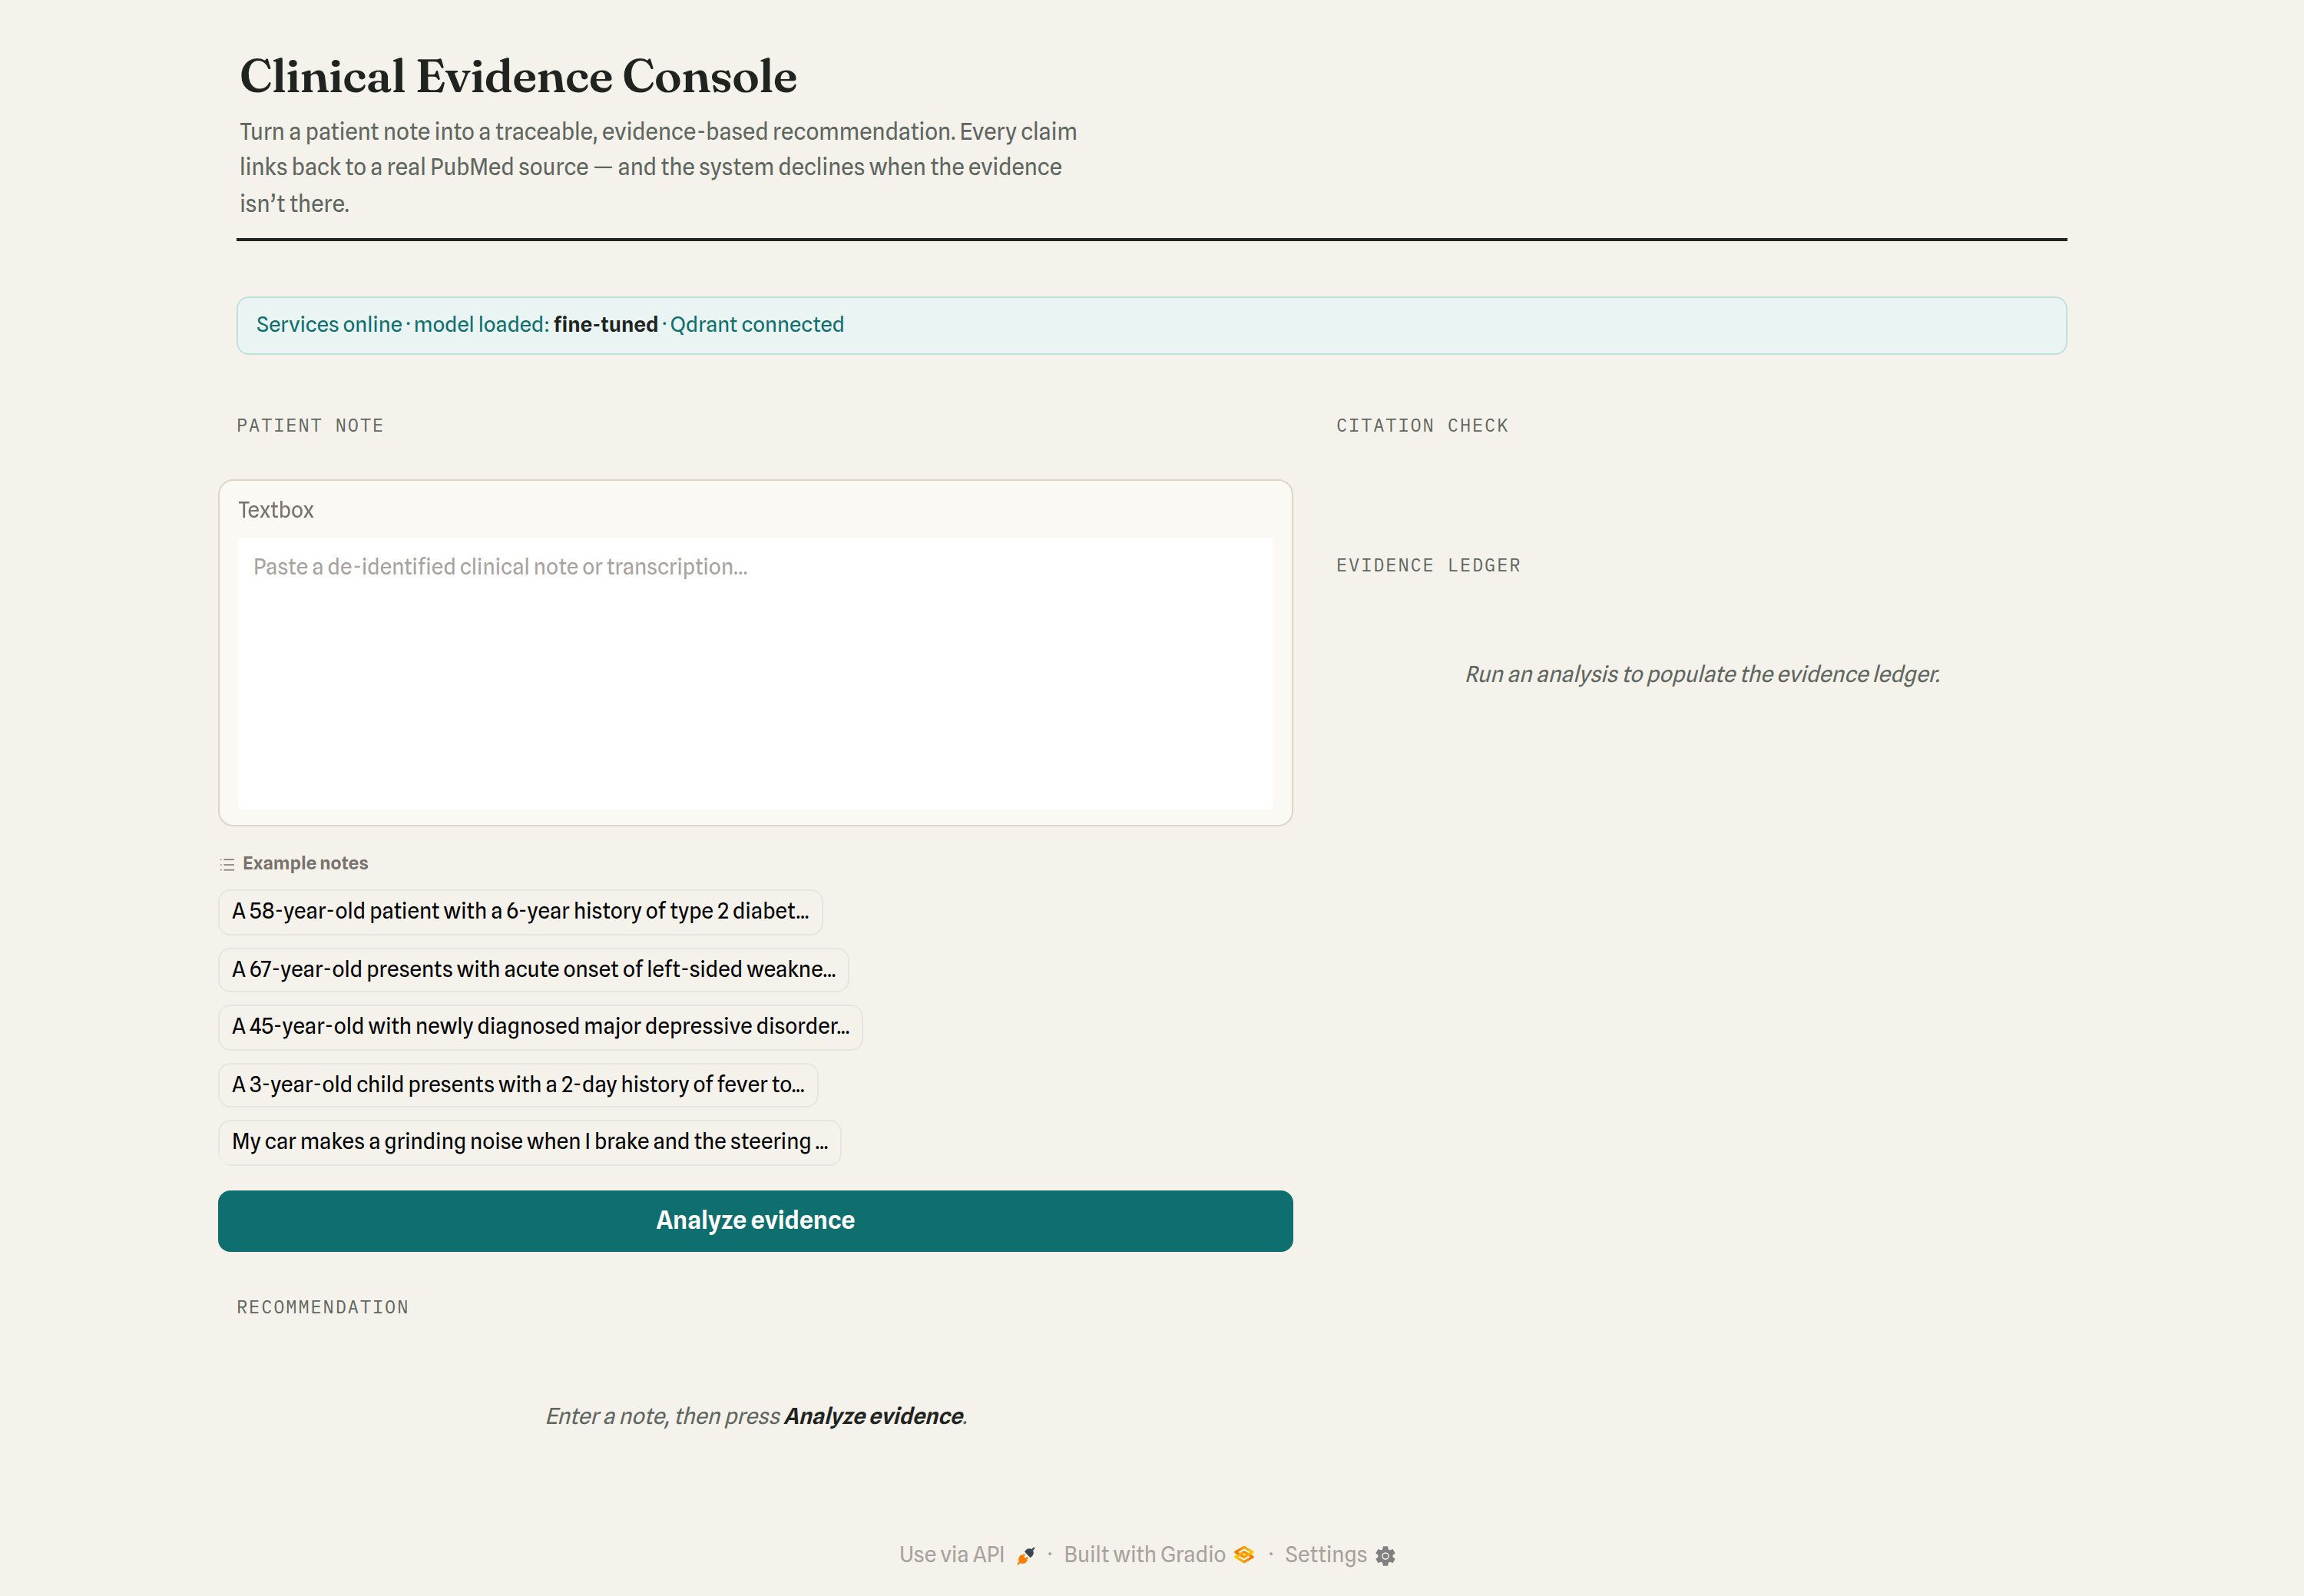
\includegraphics[width=0.85\textwidth]{figures/ui_landing.png}
\caption{Pantalla inicial de la interfaz web (Gradio), donde el clínico introduce la consulta en lenguaje natural.}
\label{fig:c5_ui_landing}
\end{figure}

\begin{figure}[h]
\centering
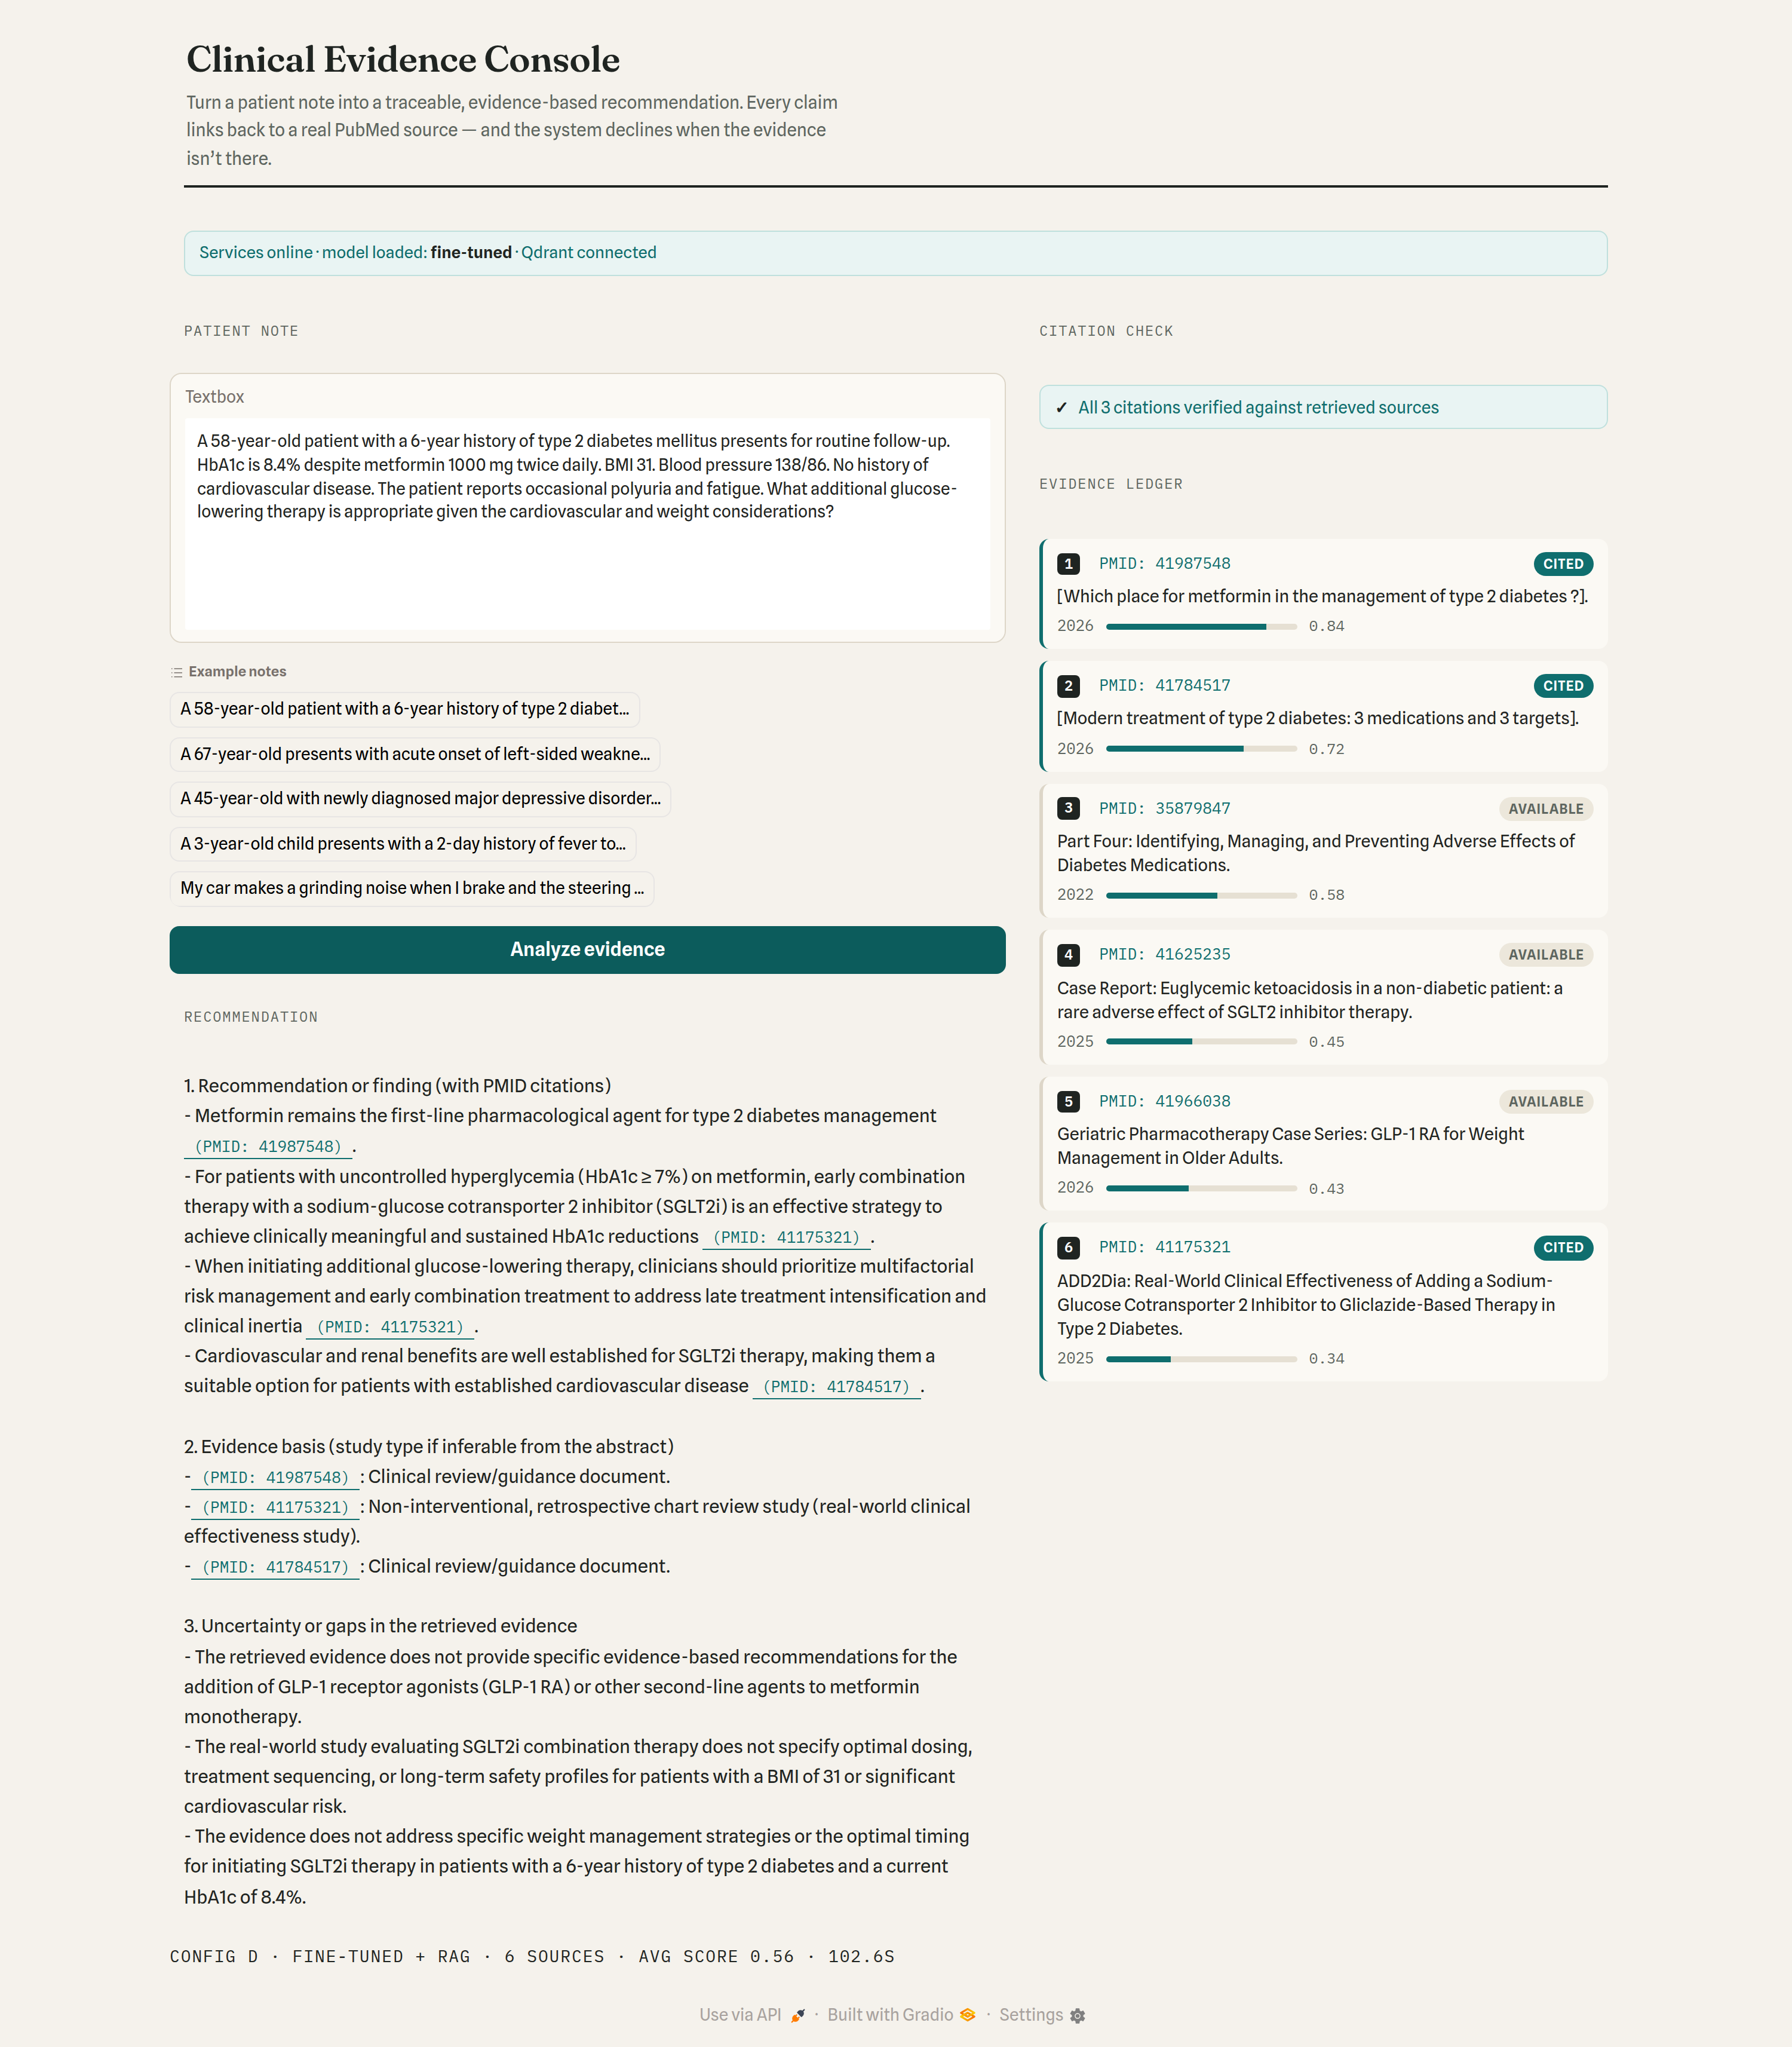
\includegraphics[width=0.85\textwidth]{figures/ui_config_d_answer.png}
\caption{Respuesta de la configuración~D (FT+RAG): la respuesta estructurada se acompaña de los abstracts de PubMed recuperados, con su PMID y un fragmento del texto (RF-09).}
\label{fig:c5_ui_answer}
\end{figure}

\begin{figure}[h]
\centering
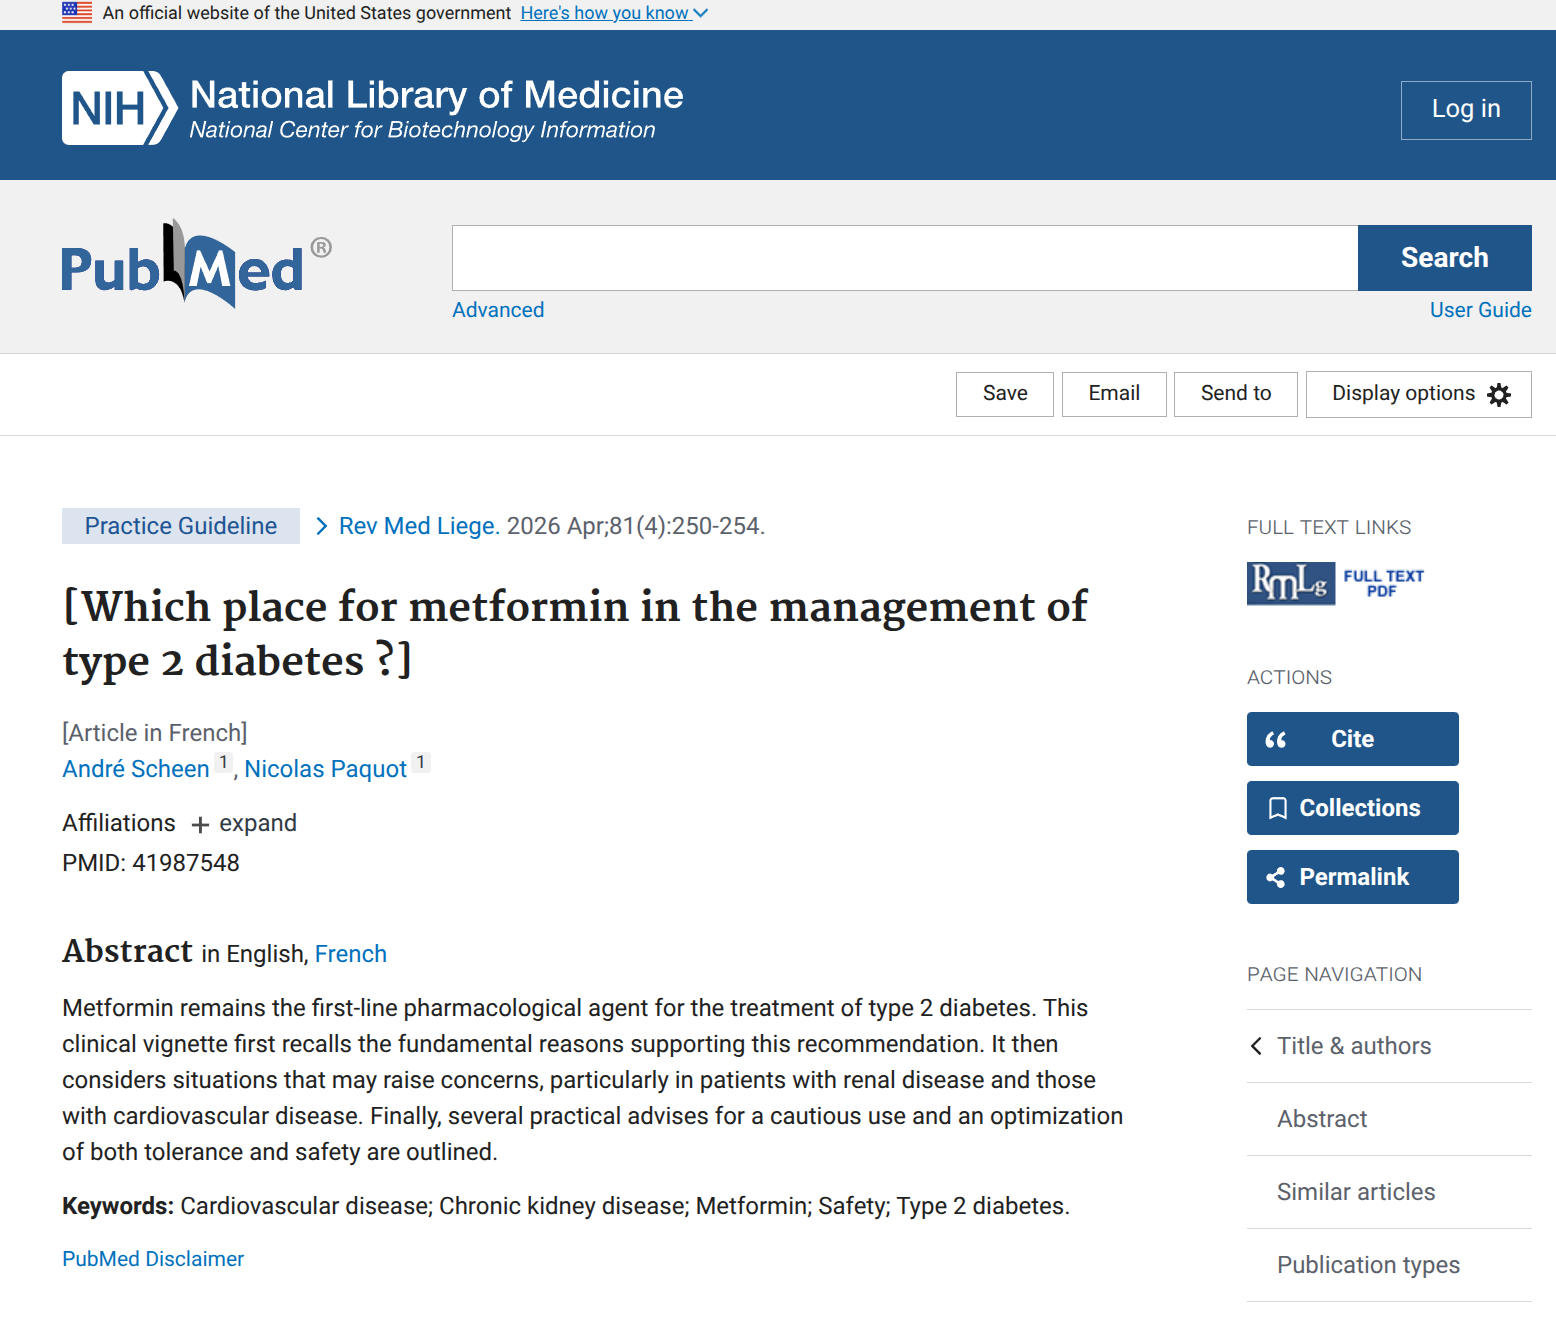
\includegraphics[width=0.85\textwidth]{figures/ui_pubmed_article.png}
\caption{Registro de PubMed (PMID~41987548) abierto al pulsar la citación correspondiente en la interfaz. La trazabilidad extremo a extremo permite contrastar cada afirmación con su fuente primaria.}
\label{fig:c5_ui_pubmed}
\end{figure}

\begin{figure}[h]
\centering
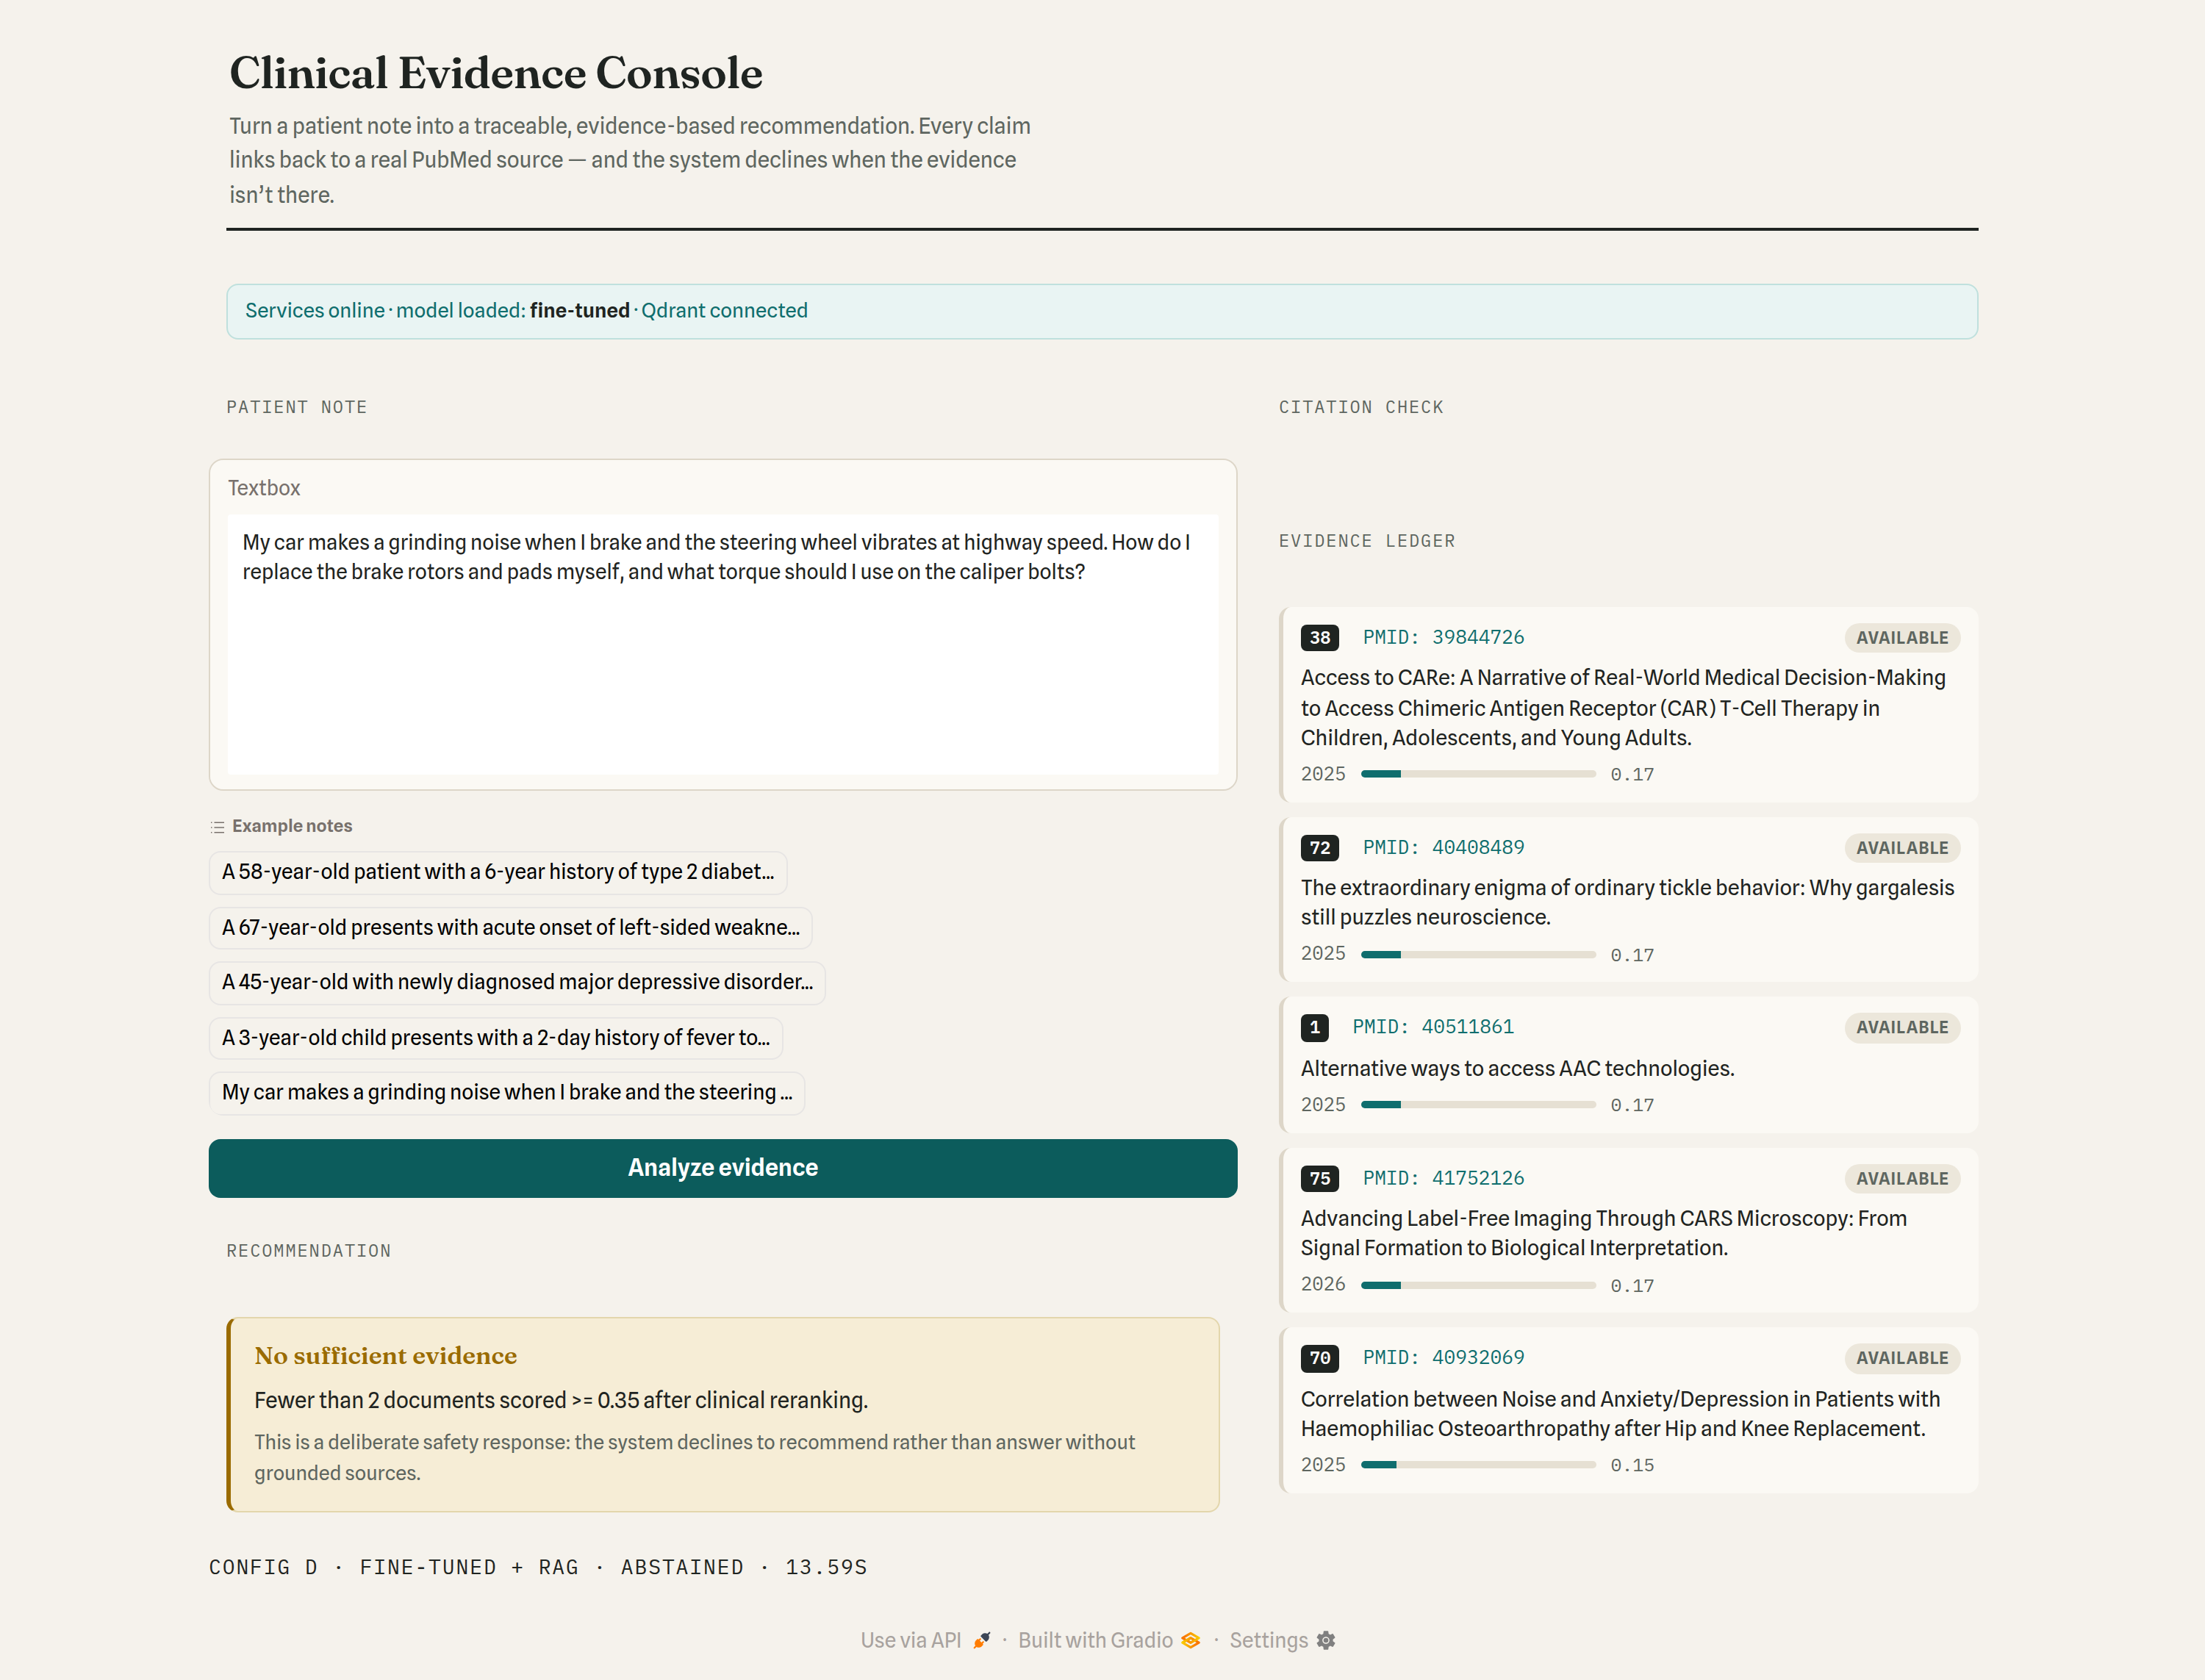
\includegraphics[width=0.85\textwidth]{figures/ui_abstention.png}
\caption{Comportamiento de abstención: ante la ausencia de evidencia recuperada suficiente, el sistema rehúsa responder en lugar de fabricar contenido.}
\label{fig:c5_ui_abstention}
\end{figure}

\chapter{Evaluación}
\label{cap:evaluacion}

Este capítulo presenta los resultados del estudio ablativo que constituye la contribución empírica central del trabajo (OE4). Se evalúan las cuatro configuraciones definidas en la Sección~\ref{sec:c5_ablation} (A: base, B: ajuste fino exclusivo, C: RAG exclusivo y D: sistema híbrido completo) sobre un mismo conjunto de consultas clínicas, combinando métricas automáticas RAGAS \cite{es2025ragasautomatedevaluationretrieval} con un conjunto de métricas deterministas de comportamiento de citación diseñadas específicamente para este estudio. El capítulo cierra con una evaluación de aplicabilidad y usabilidad de la herramienta y con la discusión de los hallazgos.

\section{Metodología de evaluación}
\label{sec:c6_metodologia}

\textbf{Muestra de evaluación.} Las cuatro configuraciones se evalúan sobre las mismas 50~notas clínicas, extraídas de la partición de test mediante muestreo estratificado por especialidad médica (\texttt{seed=42}), con los índices congelados en disco para garantizar la reproducibilidad. Se excluyen del muestreo los ejemplos sin evidencia, de modo que las métricas de calidad de respuesta midan el comportamiento del sistema cuando existe una respuesta esperable, y no casos no respondibles. La misma muestra se reutiliza en las cuatro configuraciones, por lo que las comparaciones A$\to$B, A$\to$C, B$\to$D y C$\to$D son pareadas.

\textbf{Ejecución por fases.} La restricción de servir un único modelo cuantizado en la GPU local de inferencia impone una ejecución en dos fases: la Fase~1 evalúa A~y~C con el modelo base cargado, y la Fase~2 evalúa B~y~D tras un intercambio manual al modelo con ajuste fino. La equidad de \textit{prompt} se preserva reutilizando, en las configuraciones sin RAG (A~y~B), la misma plantilla de entrenamiento con la sección de evidencia vacía (\texttt{RETRIEVED PUBMED EVIDENCE: (none)}), de forma que el modelo ajustado opera siempre sobre el andamiaje de \textit{prompt} con el que fue entrenado (Sección~\ref{sec:c5_ablation}).

\textbf{Juez y métricas RAGAS.} La evaluación automática emplea como juez a Claude Sonnet~4.6, externo al sistema bajo prueba y distinto del modelo \textit{teacher} usado en la construcción del conjunto de entrenamiento (Sección~\ref{sec:c5_sft}). Se computan las cuatro métricas RAGAS introducidas en el Capítulo~2\footnote{Las métricas que requieren contexto recuperado (\textit{faithfulness}, \textit{context precision} y \textit{context recall}) solo se definen para las configuraciones con RAG (C~y~D); para A~y~B únicamente se computa \textit{answer relevancy}.}: \textit{faithfulness} (fidelidad de la respuesta al contexto recuperado), \textit{answer relevancy} (relevancia respecto a la pregunta), \textit{context precision} y \textit{context recall} (calidad de la recuperación). Las muestras en las que el pipeline se abstiene se excluyen del denominador RAGAS y se contabilizan por separado mediante \texttt{abstention\_rate}, de modo que las puntuaciones se interpreten como ``cuando el sistema respondió, con qué calidad lo hizo''. Todas las medias se acompañan de intervalos de confianza \textit{bootstrap} del 95\,\%.

\textbf{Métricas deterministas de citación.} Las métricas RAGAS no cubren el eje de comportamiento de citación que el ajuste fino pretende inducir, y la adherencia de formato resulta saturada y poco discriminante (Sección~\ref{sec:c6_robustez}). Por ello se añade una familia de métricas deterministas, libres de juez, calculadas directamente sobre los registros de generación: la tasa de citación con PMID (\texttt{pmid\_citation\_rate}), la tasa de referencias con corchetes estilo \texttt{[1]} (\texttt{bracket\_citation\_rate}), la tasa de marcadores de posición literales \texttt{(PMID: XXXXXXXX)} (\texttt{placeholder\_citation\_rate}), la tasa de respuestas sin citación (\texttt{no\_citation\_rate}), la precisión de anclaje de las citaciones (\texttt{citation\_grounding\_precision}: fracción de PMID citados que pertenecen al conjunto recuperado de cada registro) y la tasa de alucinación de PMID por respuesta (\texttt{hallucinated\_pmids\_rate}). Estas métricas son deterministas, reproducibles sin coste de juez y miden directamente las dos hipótesis ablativas del estudio. La verificación de citaciones que las sustenta es la descrita en la Sección~\ref{sec:c5_citation}.

\section{Resultados de calidad de respuesta (RAGAS)}
\label{sec:c6_ragas}

La Tabla~\ref{tab:c6_ragas} recoge las medias RAGAS de las cuatro configuraciones sobre las 50~consultas. La Figura~\ref{fig:c6_faithfulness} representa la métrica de fidelidad con sus intervalos \textit{bootstrap}.

\begin{table}[h]
\centering
\begin{tabular}{|l|c|c|c|c|}
\hline
\textbf{Métrica RAGAS} & \textbf{A (base)} & \textbf{B (FT)} & \textbf{C (RAG)} & \textbf{D (FT+RAG)} \\
\hline
\textit{Faithfulness}      & ---       & ---       & 0{,}573         & \textbf{0{,}656} \\
\hline
\textit{Answer relevancy}  & 0{,}000   & 0{,}311   & 0{,}452         & \textbf{0{,}569} \\
\hline
\textit{Context precision} & ---       & ---       & 0{,}703         & 0{,}700 \\
\hline
\textit{Context recall}    & ---       & ---       & 0{,}938         & \textbf{0{,}947} \\
\hline
\end{tabular}
\caption{Métricas RAGAS por configuración (medias sobre los registros respondidos, $n=50$). Las métricas dependientes de contexto solo aplican a las configuraciones con RAG. En negrita, el mejor valor por fila.}
\label{tab:c6_ragas}
\end{table}

\begin{figure}[h]
\centering
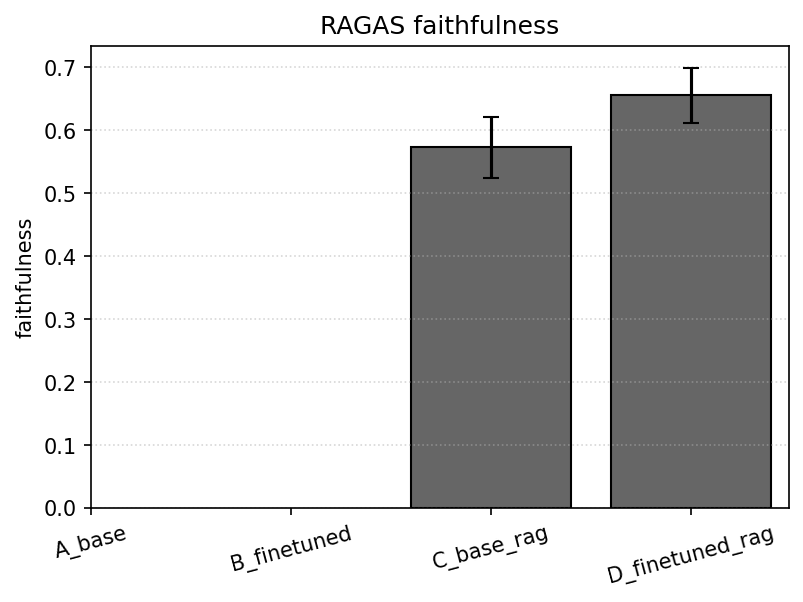
\includegraphics[width=0.7\textwidth]{figures/eval_faithfulness.png}
\caption{\textit{Faithfulness} RAGAS por configuración con IC \textit{bootstrap} del 95\,\%. Solo las configuraciones con RAG (C~y~D) reciben puntuación, al requerir esta métrica un contexto recuperado.}
\label{fig:c6_faithfulness}
\end{figure}

El hallazgo central de las métricas RAGAS es que \textbf{el ajuste fino mejora la fidelidad al combinarse con RAG}: la fidelidad asciende de 0{,}573~(C) a 0{,}656~(D), una mejora de $+0{,}083$~puntos del modelo híbrido completo sobre el RAG con modelo base. La \textit{answer relevancy} sigue la misma ordenación monótona A~$<$~B~$<$~C~$<$~D (0{,}000~$<$~0{,}311~$<$~0{,}452~$<$~0{,}569), lo que indica que ambos componentes contribuyen de forma aditiva a la relevancia de la respuesta y que su combinación (D) es la mejor configuración. La \textit{context precision} (0{,}70) y la \textit{context recall} (0{,}94--0{,}95) son prácticamente idénticas entre C~y~D, como cabe esperar, dado que ambas comparten exactamente el mismo pipeline de recuperación y solo difieren en el modelo generador; esta coincidencia confirma que las diferencias observadas en \textit{faithfulness} y \textit{answer relevancy} son atribuibles al ajuste fino del generador y no a una recuperación distinta.

La \textit{answer relevancy} de la configuración~A es de 0{,}000, valor que requiere interpretación explícita y que \textbf{no constituye un error de medición}. Ante el \textit{prompt} sin RAG (con la sección de evidencia vacía), el modelo base emite de forma sistemática la plantilla de rechazo por ausencia de evidencia en las 50~consultas; una respuesta de rechazo, por construcción, obtiene una relevancia próxima a cero respecto a la pregunta clínica concreta. Se trata, por tanto, de un hallazgo legítimo y de un contraste limpio: \emph{ante la ausencia de evidencia, el modelo base rehúsa, mientras que el modelo con ajuste fino exclusivo fabrica} (Sección~\ref{sec:c6_citacion}). El \textit{context recall} elevado (0{,}94--0{,}95) debe leerse con la cautela documentada en la metodología: la referencia de oro procede de la respuesta del \textit{teacher}, condicionada por un conjunto recuperado distinto al de la recuperación en vivo, lo que introduce un sesgo de techo; no obstante, dicho sesgo se cancela como diferencia entre C~y~D, que es la magnitud relevante para el estudio ablativo.

\section{Comportamiento de citación}
\label{sec:c6_citacion}

La Tabla~\ref{tab:c6_citacion} recoge las métricas deterministas de citación, que constituyen la evidencia principal para los dos ejes del estudio: el efecto de RAG sobre la activación de la citación y el efecto del ajuste fino sobre su formato y anclaje.

\begin{table}[h]
\centering
\begin{tabular}{|l|c|c|c|c|}
\hline
\textbf{Métrica de citación} & \textbf{A (base)} & \textbf{B (FT)} & \textbf{C (RAG)} & \textbf{D (FT+RAG)} \\
\hline
\texttt{pmid\_citation\_rate}          & 0{,}00 & 0{,}04          & 0{,}84          & \textbf{0{,}98} \\
\hline
\texttt{bracket\_citation\_rate}       & 0{,}00 & 0{,}00          & 0{,}30          & \textbf{0{,}00} \\
\hline
\texttt{placeholder\_citation\_rate}   & 0{,}00 & 0{,}60          & 0{,}00          & 0{,}00 \\
\hline
\texttt{no\_citation\_rate}            & 1{,}00 & 0{,}36          & 0{,}00          & 0{,}02 \\
\hline
\texttt{citation\_grounding\_precision}& ---    & ---             & 1{,}00          & 1{,}00 \\
\hline
\end{tabular}
\caption{Métricas deterministas de comportamiento de citación por configuración (tasas sobre registros respondidos, $n=50$). La precisión de anclaje solo se define cuando hay recuperación (C~y~D).}
\label{tab:c6_citacion}
\end{table}

\textbf{El RAG activa la citación.} La tasa de citación con PMID pasa de 0{,}00~(A) a 0{,}84~(C) y de 0{,}04~(B) a 0{,}98~(D): el componente de recuperación es el responsable de que el sistema cite literatura en absoluto. La Figura~\ref{fig:c6_pmid} ilustra este salto sobre ambos niveles del ajuste fino.

\begin{figure}[h]
\centering
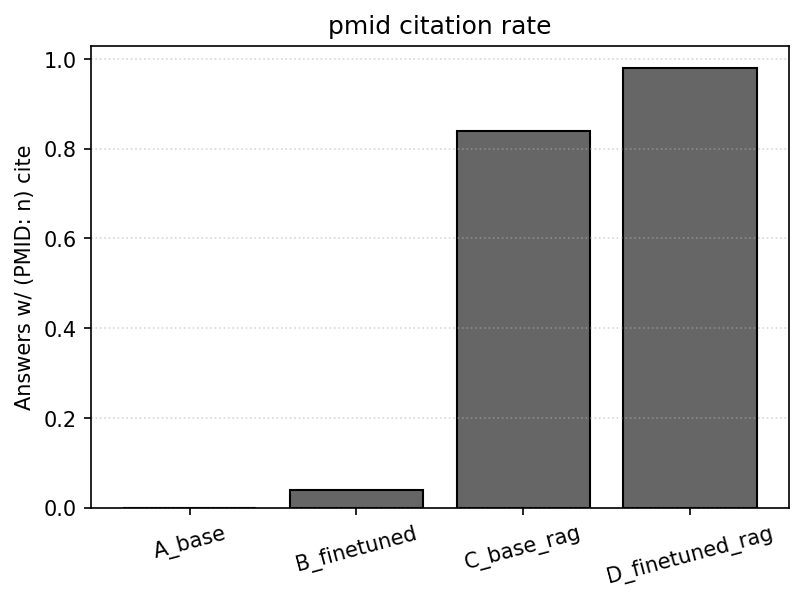
\includegraphics[width=0.7\textwidth]{figures/eval_pmid_citation_rate.png}
\caption{Tasa de citación con PMID por configuración. La recuperación (A$\to$C, B$\to$D) es la que activa la citación; el ajuste fino la lleva a la práctica totalidad de las respuestas (D, 0{,}98).}
\label{fig:c6_pmid}
\end{figure}

\textbf{El ajuste fino corrige el formato de la citación.} Sobre el sistema con RAG, el ajuste fino elimina las referencias con corchetes estilo \texttt{[1]} propias del modelo base (\texttt{bracket\_citation\_rate} de 0{,}30~en~C a 0{,}00~en~D) y eleva la citación con PMID al 0{,}98. Es decir, no solo se cita más, sino que se cita en el formato trazable y verificable \texttt{(PMID: XXXXX)} que el sistema requiere para la verificación posterior de citaciones (Sección~\ref{sec:c5_citation}). Esta es la cuantificación de un hallazgo que, de otro modo, sería meramente cualitativo: la adherencia al formato de citación es en sí misma un resultado ablativo discriminante.

\textbf{Anclaje perfecto en las configuraciones con RAG.} La precisión de anclaje (\texttt{citation\_grounding\_precision}) es de 1{,}00 tanto en C~como en~D: todos los PMID citados pertenecen al conjunto efectivamente recuperado para esa consulta. Combinado con la verificación de citaciones del pipeline (Sección~\ref{sec:c5_citation}), esto indica que, cuando se proporciona evidencia real, ninguna de las dos configuraciones con RAG cita identificadores fuera del contexto.

\textbf{Sin evidencia, el modelo base rehúsa y el modelo con ajuste fino exclusivo fabrica.} El contraste más informativo se da en las configuraciones sin RAG. La configuración~A no cita nunca (\texttt{no\_citation\_rate}~$=1{,}00$): el modelo base, ante el \textit{prompt} vacío de evidencia, rehúsa sistemáticamente. La configuración~B, en cambio, emite el marcador de posición literal \texttt{(PMID: XXXXXXXX)} en el 60\,\% de sus respuestas (Figura~\ref{fig:c6_placeholder}). Este comportamiento es \textbf{esperado y constituye en sí mismo el resultado ablativo}, no un defecto: la configuración~B recibe una entrada (\texttt{evidence = (none)}) fuera de la distribución de entrenamiento (donde siempre había documentos reales) y, al no disponer de nada legítimo que citar, reproduce el marcador de posición literal de la plantilla. La importancia de las métricas deterministas se hace aquí evidente: estas 30 de 50~respuestas con marcador de posición obtenían una adherencia de formato del 100\,\% y una alucinación nula bajo las métricas previas, que eran ciegas a este patrón. El marcador de posición no es un PMID con dígitos y, por tanto, no se contabiliza como alucinación; representa una fabricación de forma sin contenido, distinta de inventar un identificador concreto.

\begin{figure}[h]
\centering
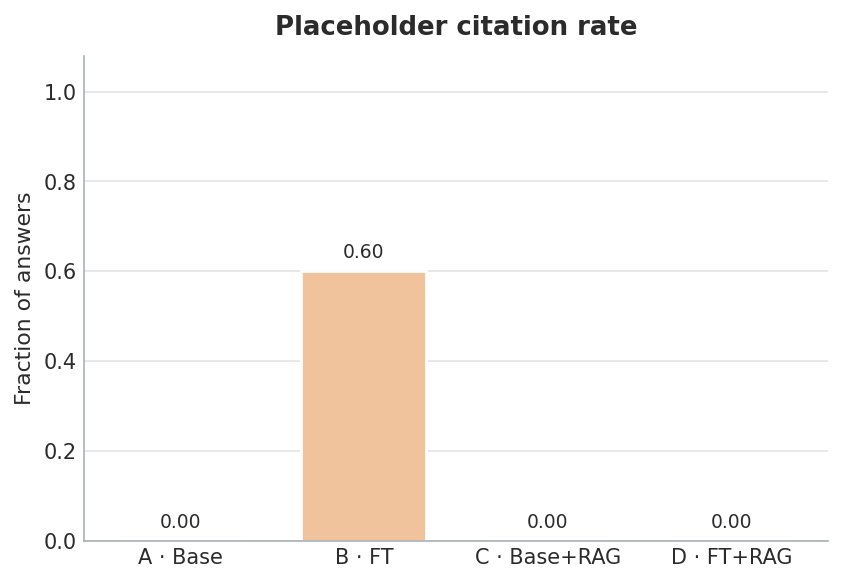
\includegraphics[width=0.7\textwidth]{figures/eval_placeholder_cite.png}
\caption{Tasa de marcadores de posición literales \texttt{(PMID: XXXXXXXX)} por configuración. Solo la configuración~B (ajuste fino sin RAG) los produce, al operar fuera de su distribución de entrenamiento sin evidencia que citar.}
\label{fig:c6_placeholder}
\end{figure}

\section{Alucinación de PMID y robustez operativa}
\label{sec:c6_robustez}

La Tabla~\ref{tab:c6_robustez} recoge las métricas de alucinación y de robustez operativa. La tasa de alucinación de PMID (fracción de respuestas con al menos un PMID inventado, es decir, con dígitos pero ausente del conjunto recuperado) es muy baja en todas las configuraciones: 0{,}00~(A), 0{,}04~(B), 0{,}00~(C) y 0{,}02~(D). El valor de la configuración~D (0{,}02, un único caso) confirma que el sistema híbrido completo casi nunca fabrica identificadores numéricos, en línea con su precisión de anclaje de 1{,}00. La alucinación de la configuración~B (0{,}04) es modesta porque su modo de fallo dominante no es inventar dígitos, sino reproducir el marcador de posición de la plantilla, que la Sección~\ref{sec:c6_citacion} captura por separado.

\begin{table}[h]
\centering
\begin{tabular}{|l|c|c|c|c|}
\hline
\textbf{Métrica} & \textbf{A (base)} & \textbf{B (FT)} & \textbf{C (RAG)} & \textbf{D (FT+RAG)} \\
\hline
\texttt{hallucinated\_pmids\_rate} & 0{,}00 & 0{,}04 & 0{,}00 & 0{,}02 \\
\hline
\texttt{abstention\_rate}         & 0{,}00 & 0{,}00 & 0{,}00 & 0{,}00 \\
\hline
\texttt{error\_rate}              & 0{,}00 & 0{,}00 & 0{,}00 & 0{,}00 \\
\hline
\texttt{format\_adherence}        & 1{,}00 & 1{,}00 & 1{,}00 & 1{,}00 \\
\hline
\end{tabular}
\caption{Métricas de alucinación y robustez operativa por configuración ($n=50$).}
\label{tab:c6_robustez}
\end{table}

La tasa de abstención es de 0{,}00 en las dos configuraciones que pueden abstenerse (C~y~D): el pipeline de recuperación superó la puerta de abstención (al menos dos documentos por encima del umbral \texttt{min\_final\_score}) en las 50~consultas, lo que es coherente con haber excluido del muestreo los casos sin evidencia. La tasa de error es nula en las cuatro configuraciones: ninguna generación falló durante las dos fases del estudio. La adherencia de formato satura en 1{,}00 en todas las configuraciones (como se anticipó), lo que la convierte en una métrica poco discriminante: incluso la plantilla de rechazo de A y los marcadores de posición de B satisfacen la comprobación estructural. Es precisamente esta saturación la que motivó la introducción de las métricas deterministas de citación, capaces de distinguir comportamientos que la adherencia de formato agrega indistintamente.

\section{Evaluación de aplicabilidad y usabilidad}
\label{sec:c6_usabilidad}

Por su tipología, este trabajo de desarrollo de software requiere, además de la evaluación cuantitativa anterior, una valoración de la aplicabilidad de la herramienta para resolver el problema propuesto y una evaluación mínima de su usabilidad. Esta sección cubre ambos aspectos.

\textbf{Aplicabilidad.} La aplicabilidad del sistema para la asistencia bibliográfica clínica queda demostrada por el propio estudio ablativo. La configuración híbrida completa (D) responde a las 50~consultas clínicas sin errores ni abstenciones (Tabla~\ref{tab:c6_robustez}), cita literatura primaria real de PubMed en el 98\,\% de las respuestas (Tabla~\ref{tab:c6_citacion}) con una precisión de anclaje del 100\,\% (ningún identificador citado queda fuera de la evidencia recuperada) y mejora la fidelidad y la relevancia frente a las configuraciones parciales (Tabla~\ref{tab:c6_ragas}). El sistema cumple, por tanto, su función prevista sobre el conjunto de evaluación: producir respuestas clínicas estructuradas y trazables ancladas en evidencia verificable.

\textbf{Usabilidad: evaluación heurística del autor.} La validación cualitativa de usabilidad con un profesional sanitario quedó condicionada, ya en la Sección~\ref{sec:c4_validacion}, a la disponibilidad de dicha colaboración dentro del calendario del trabajo. Al no resultar posible, y conforme a la alternativa allí prevista, la usabilidad se valora mediante una revisión heurística documentada por el autor. Esta revisión examina la interfaz web (Gradio) y el flujo de interacción que ofrece, tomando como referencia un subconjunto de los principios heurísticos de usabilidad y anclando cada principio en funcionalidades del sistema efectivamente implementadas y evaluadas en los apartados anteriores. La Tabla~\ref{tab:c6_heuristica} resume esta valoración.

\begin{table}[h]
\centering
\begin{tabular}{|p{0.30\textwidth}|p{0.60\textwidth}|}
\hline
\textbf{Principio heurístico} & \textbf{Soporte en el sistema} \\
\hline
Visibilidad del estado del sistema & La interfaz muestra explícitamente un indicador de estado del servicio (modelo de generación activo y disponibilidad de la recuperación) y, junto a cada respuesta, los \textit{abstracts} recuperados con su PMID y un fragmento del texto (RF-09). \\
\hline
Control y libertad del usuario & El usuario reformula libremente la consulta en lenguaje natural y dispone de notas de ejemplo para iniciar el análisis; ante evidencia insuficiente, el sistema responde con un estado explícito de abstención en lugar de fabricar una recomendación, manteniendo al usuario en control del proceso. \\
\hline
Reconocer en lugar de recordar & Las fuentes se presentan junto a la respuesta, de modo que el usuario puede verificar la evidencia sin abandonar la interfaz ni memorizar identificadores. \\
\hline
Prevención de errores & La puerta de abstención y el verificador de citaciones (Secciones~\ref{sec:c5_clinical_scorer} y~\ref{sec:c5_citation}) evitan que el sistema emita respuestas sin evidencia suficiente o con citas no ancladas en el contexto recuperado. \\
\hline
Coincidencia con el dominio real & El ajuste fino adapta la terminología y la estructura de la respuesta (recomendación / base de evidencia / incertidumbre) al registro clínico, como evidencian las métricas de formato y citación. \\
\hline
\end{tabular}
\caption{Evaluación heurística de usabilidad realizada por el autor, anclada en funcionalidades implementadas y evaluadas.}
\label{tab:c6_heuristica}
\end{table}

Esta evaluación heurística es una valoración del autor y no sustituye a un estudio empírico de usabilidad con usuarios reales. Sus limitaciones (ausencia de profesionales sanitarios y de métricas de interacción: tiempo de tarea, tasa de éxito, satisfacción percibida) se asumen explícitamente, y la realización de una sesión de evaluación con al menos un experto del dominio clínico, sobre la interfaz ya integrada, se identifica como línea prioritaria de trabajo futuro (Capítulo~7).

\section{Análisis cualitativo de respuestas representativas}
\label{sec:c6_cualitativo}

Las métricas anteriores resumen el comportamiento agregado de las cuatro configuraciones, pero no permiten \emph{ver} las diferencias que cuantifican. Esta sección las hace explícitas mediante un caso representativo del conjunto de evaluación, en el que las cuatro configuraciones responden a la misma consulta clínica. Por tratarse de comparaciones pareadas sobre idéntica entrada (Sección~\ref{sec:c6_metodologia}), el contraste cualitativo aísla el efecto de cada componente con la misma limpieza que las métricas.

El caso seleccionado (especialidad \textit{Orthopedic}) corresponde a una nota operatoria de reparación de un desgarro del manguito rotador con descompresión subacromial artroscópica. La Tabla~\ref{tab:c6_cualitativo} recoge un extracto de la respuesta de cada configuración, centrado en su comportamiento de citación. El extracto reproduce literalmente la salida del modelo; las elisiones se indican con \textnormal{[\ldots]}.

\begin{table}[h]
\centering
\small
\renewcommand{\arraystretch}{1.3}
\begin{tabular}{|p{0.16\textwidth}|p{0.74\textwidth}|}
\hline
\textbf{Configuración} & \textbf{Extracto de la respuesta} \\
\hline
\textbf{A (base)} & \emph{«The retrieved context is off-topic or insufficient for this clinical case. [\ldots] no evidence-based recommendation can be made from the provided documents.»} \par\smallskip {\footnotesize\itshape Conclusión: rehúsa por considerar el contexto insuficiente y no emite ninguna recomendación.} \\
\hline
\textbf{B (FT)} & \emph{«Arthroscopic subacromial decompression combined with rotator cuff repair via mini-arthrotomy is an evidence-based treatment [\ldots]} \texttt{(PMID: XXXXXXXX)}\emph{. [\ldots] As no peer-reviewed PubMed evidence was provided, no PMID citations can be supplied.»} \par\smallskip {\footnotesize\itshape Conclusión: recomendación bien estructurada, pero cita el marcador de posición vacío y admite no poder aportar ningún PMID.} \\
\hline
\textbf{C (RAG)} & \emph{«Transosseous suture technique is a possible improvement in the surgical repair of the rotator cuff [\ldots]. The rate of infection after mini-open rotator cuff repair is low, approximately 1.7\%. [\ldots] Evidence basis:} \texttt{[1]} \emph{Prospective study [\ldots];} \texttt{[4]} \emph{Randomized controlled trial comparing [\ldots] transosseous hardware-free suture repair;} \texttt{[5]} \emph{Retrospective study evaluating the rate of infection after mini-open rotator cuff repair.»} \par\smallskip {\footnotesize\itshape Conclusión: sintetiza evidencia real (sutura transósea, tasa de infección del 1{,}7\,\%) pero la referencia con corchetes no trazables.} \\
\hline
\textbf{D (FT+RAG)} & \emph{«Arthroscopic rotator cuff repair utilizing a transosseous suture technique is a viable surgical option [\ldots], with the added benefit of reduced postoperative pain} \texttt{(PMID: 28339286)}\emph{. The mini-open rotator cuff repair technique is a safe and effective alternative [\ldots], with a low overall infection rate (1.7\%) [\ldots]} \texttt{(PMID: 39384012)}\emph{.»} \par\smallskip {\footnotesize\itshape Conclusión: la misma evidencia que C, pero anclada a PMID reales y verificables.} \\
\hline
\end{tabular}
\caption{Extractos de las respuestas de las cuatro configuraciones a una misma consulta clínica (manguito rotador, especialidad \textit{Orthopedic}). Se conserva el texto original en inglés y se resaltan en \texttt{monoespaciado} los marcadores de citación.}
\label{tab:c6_cualitativo}
\end{table}

El extracto materializa los hallazgos cuantitativos de las secciones anteriores. La configuración~A rehúsa ante la ausencia de evidencia recuperada (\texttt{no\_citation\_rate}~$=1{,}00$). La configuración~B produce una respuesta estructuralmente correcta pero emite el marcador de posición literal \texttt{(PMID: XXXXXXXX)} (reconociendo incluso, en el mismo texto, que «no PMID citations can be supplied»), ilustrando la fabricación de forma sin contenido descrita en la Sección~\ref{sec:c6_citacion}. El contraste más revelador se da entre C~y~D: ambas disponen de la misma evidencia recuperada y mencionan los mismos hechos clínicos (la técnica de sutura transósea, la tasa de infección del 1{,}7\,\% en la reparación mini-open), pero C los referencia con marcadores de corchete estilo \texttt{[1]}, \texttt{[4]}, \texttt{[5]} que no son trazables, mientras que D los ancla a PMID reales y verificables (\texttt{28339286}, \texttt{39384012}). Es la evidencia visual directa de que la recuperación aporta el contenido y el ajuste fino disciplina su formato de citación. En el Anexo~\ref{anexo:cualitativo} se recogen dos ejemplos adicionales, de otras especialidades, con las respuestas completas.

\section{Discusión de los hallazgos}
\label{sec:c6_discusion}

\textbf{Cumplimiento de los criterios de éxito.} El objetivo general (Capítulo~3) y el requisito RNF-07 fijaron dos criterios cuantitativos relativos al \textit{baseline}. El primero (que la configuración FT+RAG (D) supere a la base (A) en al menos $0{,}10$ puntos de \textit{answer relevancy}) \textbf{se cumple con amplio margen}: la diferencia es de $0{,}569 - 0{,}000 = +0{,}569$. El segundo, relativo a \textit{faithfulness}, requiere una matización honesta: esta métrica solo es computable cuando existe contexto recuperado, por lo que \emph{no está definida para la configuración base} (A, sin RAG) y el único eje sobre el que es comparable es C$\to$D. En ese eje, el ajuste fino mejora la fidelidad en $+0{,}083$~puntos (0{,}573~$\to$~0{,}656): una mejora positiva y consistente con la hipótesis, que aísla la contribución del ajuste fino a la fidelidad, aunque queda ligeramente por debajo del umbral de $0{,}10$ que se barajó en una formulación inicial del criterio. Se reporta, por tanto, sin redondeos favorables: la dirección y el signo del efecto respaldan la hipótesis, y su magnitud exacta ($+0{,}083$) se documenta tal cual.

Los resultados permiten separar de forma limpia las contribuciones de cada componente, en línea con la literatura comparativa de RAG frente a ajuste fino en dominios especializados \cite{balaguer2024ragvsfinetuningpipelines, ovadia2024finetuningretrievalcomparingknowledge, pingua_medical_FT_vs_RAG_2025}:

\begin{itemize}
  \item \textbf{La recuperación (RAG) aporta la evidencia y activa la citación.} Es la condición necesaria para que el sistema cite literatura real: sin RAG, ninguna configuración cita PMID legítimos. RAG es además el responsable de poder computar fidelidad y precisión de contexto, ejes inexistentes sin evidencia recuperada \cite{lewis_retrieval-augmented_2021}.
  \item \textbf{El ajuste fino disciplina el comportamiento.} Sobre el sistema con RAG, corrige el formato de citación (elimina las referencias \texttt{[1]} del modelo base y lleva la citación con PMID al 0{,}98), mejora la fidelidad ($+0{,}083$) y la relevancia de la respuesta. Confirma que el ajuste fino actúa como alineamiento de comportamiento y no como inyección de conocimiento, en coherencia con el diseño de la Sección~\ref{sec:c5_sft}.
  \item \textbf{Los dos componentes son complementarios y su combinación (D) es óptima.} La configuración híbrida completa domina en \textit{faithfulness} (0{,}656), \textit{answer relevancy} (0{,}569), tasa de citación con PMID (0{,}98) y precisión de anclaje (1{,}00), validando la hipótesis central del trabajo.
  \item \textbf{El ajuste fino sin recuperación es frágil ante la ausencia de evidencia.} La configuración~B revela el riesgo de desplegar un modelo ajustado sin su pipeline de recuperación: fuera de distribución, fabrica la forma de una citación (marcador de posición en el 60\,\% de los casos) en lugar de rehusar. Esto refuerza, desde la evidencia empírica, la necesidad del componente RAG en producción y la pertinencia de la puerta de abstención y la verificación de citaciones como salvaguardas \cite{ji_survey_2023, pal_med-halt_2023}.
\end{itemize}

\section{Amenazas a la validez y limitaciones}
\label{sec:c6_limitaciones}

El estudio presenta varias limitaciones que se documentan en aras del rigor:

\begin{itemize}
  \item \textbf{Tamaño muestral.} La evaluación se realiza sobre 50~consultas por configuración, dimensionadas por el coste temporal de la inferencia local y del juzgado RAGAS. Las medias se reportan con intervalos \textit{bootstrap} del 95\,\% para acotar la incertidumbre, pero las diferencias de menor magnitud (por ejemplo, \textit{context recall} 0{,}938 frente a 0{,}947) deben interpretarse como equivalentes dentro del ruido muestral.
  \item \textbf{Ausencia de benchmark IR con anotación de oro.} La selección del modelo de embeddings se sustenta en el proxy de categoría MeSH (Sección~\ref{sec:c5_embedding}) y no en un conjunto anotado de relevancia, cuyo coste de anotación excede el alcance del trabajo. Las métricas RAGAS de contexto miden la calidad de recuperación de forma comparativa, no absoluta.
  \item \textbf{Techo del \textit{context recall}.} La referencia de oro derivada del \textit{teacher} introduce un sesgo de techo en \textit{context recall}, mitigado al interpretarse como diferencia entre C~y~D (sesgo común que se cancela).
  \item \textbf{Usabilidad sin usuarios reales.} La evaluación de usabilidad es una revisión heurística del autor; carece de validación con profesionales sanitarios y de métricas de interacción, lo que se aborda como trabajo futuro (Sección~\ref{sec:c6_usabilidad}).
  \item \textbf{Determinismo procedimental.} La reproducibilidad es procedimental (configuración fijada, \texttt{seed=42}, \textit{hash} de dataset e hiperparámetros registrados en MLflow) y no bit a bit entre distinto hardware, por el entrenamiento en GPU en la nube y la inferencia local cuantizada (Sección~\ref{sec:c5_qlora}).
\end{itemize}

\chapter{Conclusiones y Trabajo Futuro}

%En la Ecuación \eqref{eq:eq1secCTF}


%\begin{equation}\label{eq:eq1secCTF}
%M=\begin{pmatrix}
%	m_{11}&m_{12}\\
%	m_{21}&m_{22}
%\end{pmatrix}
%\end{equation}

%En la siguiente Tabla \ref{tab:tab1secCTF}

%\begin{table}[h]
%\centering
%\begin{tabular}{|c|c|}
%	\hline
%	1 & 2 \\
%	\hline
%	22 & 11 \\
%	\hline
%\end{tabular}
%\caption{Tabla 1}
%\label{tab:tab1secCTF}
%\end{table}

%En la siguiente Figura \ref{fig:fig1secCTF}

%\begin{figure}[h]
%
\includegraphics[width= 0.8\textwidth]{logo_unir}
%\caption{Logo Unir}
%\label{fig:fig1secCTF}
%\end{figure}


%\begin{thebibliography}{a}
%\bibitem{etiqueta} \textsc{Autores},
%\textit{nombre referencia.}
%Información addicional
%\end{thebibliography}
\bibliographystyle{apacite}
\bibliography{bibliografia}

\appendix
\chapter{Resultados de evaluación detallados}
\label{anexo:eval}

Este anexo recoge la tabla completa de métricas del estudio ablativo (Capítulo~\ref{cap:evaluacion}) y las figuras comparativas que complementan a las incluidas en el cuerpo del capítulo. Todos los valores proceden de las ejecuciones registradas en MLflow (experimento \texttt{tfm-evaluation}), con $n=50$ consultas por configuración.

\begin{table}[h]
\centering
\small
\begin{tabular}{|l|c|c|c|c|}
\hline
\textbf{Métrica} & \textbf{A (base)} & \textbf{B (FT)} & \textbf{C (RAG)} & \textbf{D (FT+RAG)} \\
\hline
\textit{faithfulness} (RAGAS)        & ---     & ---     & 0{,}573 & 0{,}656 \\
\textit{answer relevancy} (RAGAS)    & 0{,}000 & 0{,}311 & 0{,}452 & 0{,}569 \\
\textit{context precision} (RAGAS)   & ---     & ---     & 0{,}703 & 0{,}700 \\
\textit{context recall} (RAGAS)      & ---     & ---     & 0{,}938 & 0{,}947 \\
\hline
\texttt{pmid\_citation\_rate}          & 0{,}00 & 0{,}04 & 0{,}84 & 0{,}98 \\
\texttt{bracket\_citation\_rate}       & 0{,}00 & 0{,}00 & 0{,}30 & 0{,}00 \\
\texttt{placeholder\_citation\_rate}   & 0{,}00 & 0{,}60 & 0{,}00 & 0{,}00 \\
\texttt{no\_citation\_rate}            & 1{,}00 & 0{,}36 & 0{,}00 & 0{,}02 \\
\texttt{citation\_grounding\_precision}& ---    & ---    & 1{,}00 & 1{,}00 \\
\hline
\texttt{hallucinated\_pmids\_rate}     & 0{,}00 & 0{,}04 & 0{,}00 & 0{,}02 \\
\texttt{abstention\_rate}              & 0{,}00 & 0{,}00 & 0{,}00 & 0{,}00 \\
\texttt{error\_rate}                   & 0{,}00 & 0{,}00 & 0{,}00 & 0{,}00 \\
\texttt{format\_adherence}             & 1{,}00 & 1{,}00 & 1{,}00 & 1{,}00 \\
\hline
\end{tabular}
\caption{Tabla completa de métricas del estudio ablativo por configuración ($n=50$). Las celdas «---» indican métricas no definidas para esa configuración (las métricas RAGAS dependientes de contexto y la precisión de anclaje solo aplican a las configuraciones con RAG).}
\label{tab:anexo_eval_full}
\end{table}

\begin{figure}[h]
\centering
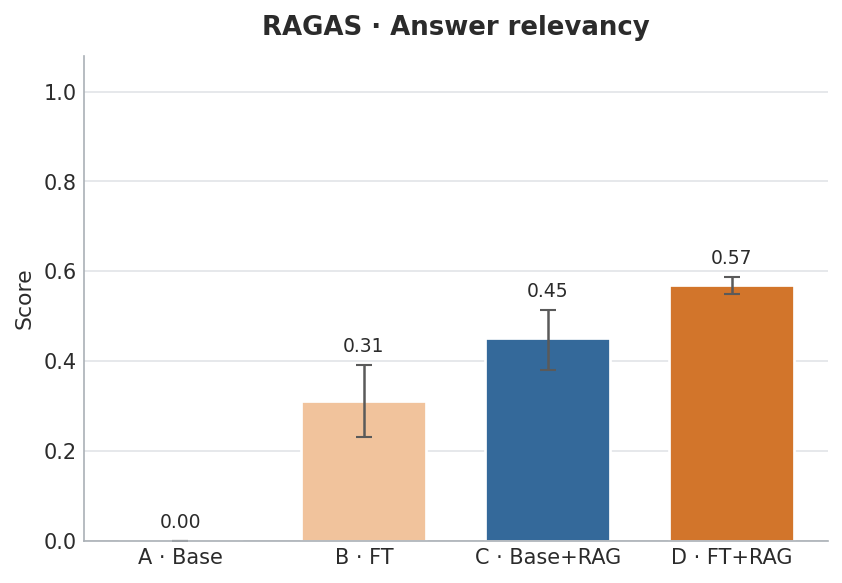
\includegraphics[width=0.48\textwidth]{figures/eval_answer_relevancy.png}
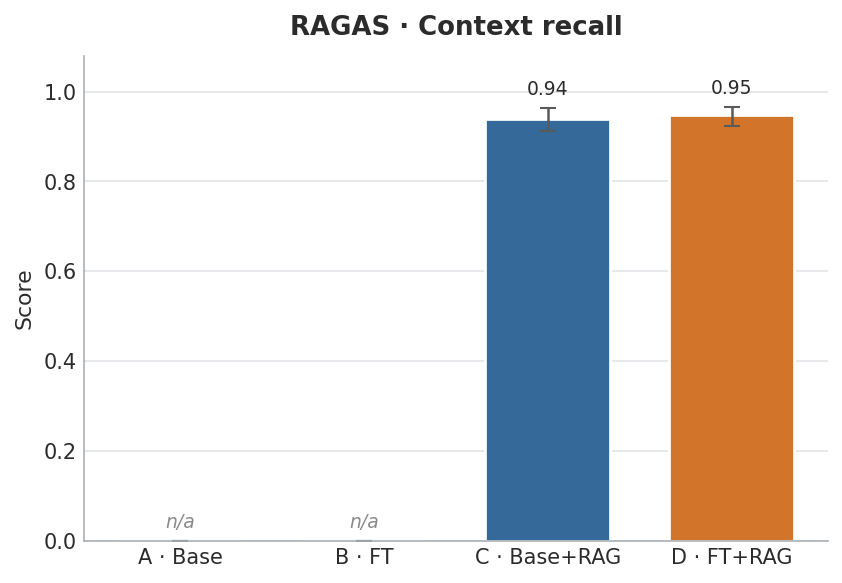
\includegraphics[width=0.48\textwidth]{figures/eval_context_recall.png}
\\[0.5em]
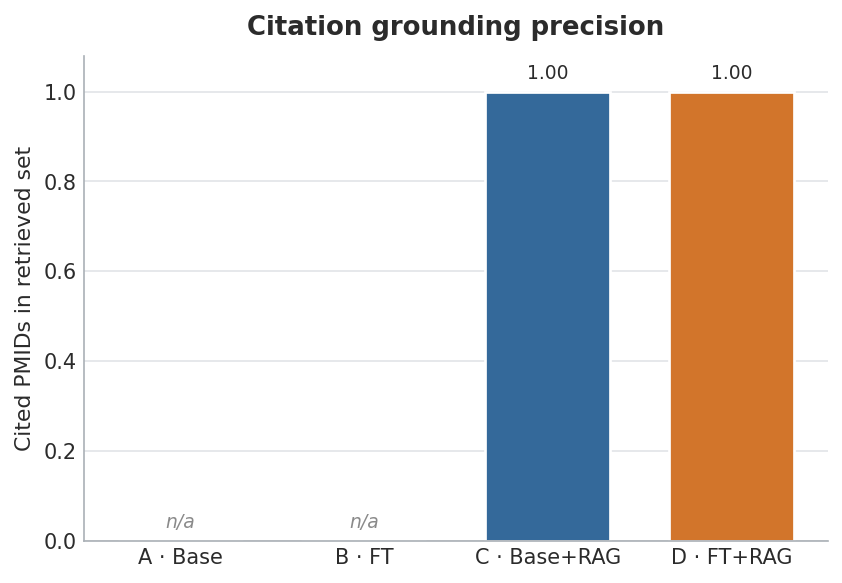
\includegraphics[width=0.48\textwidth]{figures/eval_grounding_precision.png}
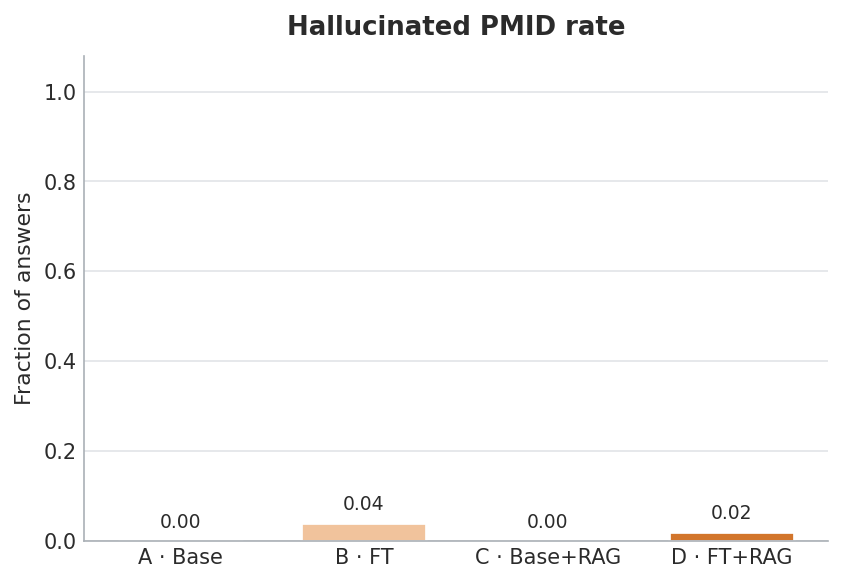
\includegraphics[width=0.48\textwidth]{figures/eval_hallucinated_pmids.png}
\caption{Figuras comparativas complementarias por configuración (con IC \textit{bootstrap} del 95\,\% donde aplica): \textit{answer relevancy} y \textit{context recall} (RAGAS), precisión de anclaje de citaciones y tasa de alucinación de PMID.}
\label{fig:anexo_eval_grid}
\end{figure}

\chapter{Ejemplos cualitativos de respuestas por configuración}
\label{anexo:cualitativo}

Este anexo complementa el ejemplo representativo de la Sección~\ref{sec:c6_cualitativo} con dos casos adicionales del conjunto de evaluación, de especialidades distintas, en los que se reproducen las respuestas completas de las cuatro configuraciones a una misma consulta. Se conserva el texto original en inglés generado por el sistema; los marcadores de citación (\texttt{(PMID:~XXXXXXXX)}, corchetes \texttt{[n]} y PMID reales) se resaltan en monoespaciado. El objetivo es evidenciar que los patrones cuantificados en el Capítulo~\ref{cap:evaluacion} (rechazo de la configuración~A, marcador de posición de la~B, referencias no trazables de la~C y citación anclada de la~D) se reproducen de forma consistente entre especialidades.

\section{Ejemplo 1: cirugía abdominal (hernia incisional y cuerpo extraño retenido)}
\label{anexo:cualitativo_ej1}

\textbf{Consulta (resumen).} Nota operatoria de un paciente con quiste sebáceo de abdomen recurrentemente infectado, absceso secundario a cuerpo extraño retenido y hernia incisional; procedimientos de excisión del absceso, retirada del cuerpo extraño y reparación de la hernia.

\begin{quote}\small
\textbf{A (base).} \emph{«The retrieved context is off-topic or insufficient for this clinical case. [\ldots] No evidence-based recommendation can be made from the provided documents.»}
\end{quote}
\noindent{\footnotesize\itshape Conclusión: rehúsa por considerar el contexto insuficiente y no emite ninguna recomendación.}

\begin{quote}\small
\textbf{B (FT).} \emph{«Excision of the infected cyst and hernia repair are appropriate surgical interventions for recurrently infected sebaceous cysts and associated hernias.} \texttt{(PMID: XXXXXXXX)}\emph{. [\ldots] This recommendation is derived from a single patient note/case report [\ldots]. The retrieved evidence consists solely of a clinical operative note and lacks peer-reviewed literature [\ldots]; consequently, no evidence-based recommendation can be made.»}
\end{quote}
\noindent{\footnotesize\itshape Conclusión: recomendación estructurada con marcador de posición vacío; reconoce la ausencia de literatura revisada por pares.}

\begin{quote}\small
\textbf{C (RAG).} \emph{«Use of monofilament sutures may reduce the risk of incisional hernia} \texttt{(PMID: 29099149)}\emph{. Absorbable sutures may reduce the risk of sinus or fistula tract formation} \texttt{(PMID: 29099149)}\emph{. Transfascial suture fixation technique (TRANSFIX) appears to be a safe and economical mesh fixation method for laparoscopic inguinal hernia repair} \texttt{(PMID: 31099180)}\emph{. Incisional negative pressure wound therapy (iNPWT) may be beneficial in preventing wound healing disorders [\ldots]} \texttt{(PMID: 34110077)}\emph{. Evidence basis: Systematic review and meta-analysis} \texttt{(PMID: 29099149)}\emph{; Case series} \texttt{(PMID: 31099180)}\emph{; Retrospective analysis} \texttt{(PMID: 34110077)}\emph{.»}
\end{quote}
\noindent{\footnotesize\itshape Conclusión: cita PMID reales sobre suturas, fijación de malla y terapia de presión negativa, con el tipo de estudio de cada fuente.}

\begin{quote}\small
\textbf{D (FT+RAG).} \emph{«For abdominal wall closure following laparotomy, monofilament sutures are recommended to reduce the risk of incisional hernia formation} \texttt{(PMID: 29099149)}\emph{. The use of incisional negative pressure wound therapy (iNPWT) may be considered as a preventive measure to mitigate wound healing impairments and surgical site infections [\ldots]} \texttt{(PMID: 34110077)}\emph{. Retained surgical foreign bodies, including gossypibomas, should be recognized as a preventable complication and managed with prompt surgical removal [\ldots]} \texttt{(PMID: 39438894)}\emph{. [\ldots] The recommendation for monofilament sutures is based on a systematic review and meta-analysis of 55 randomized controlled trials involving 19,174 participants} \texttt{(PMID: 29099149)}\emph{.»}
\end{quote}
\noindent{\footnotesize\itshape Conclusión: refina la evidencia e incorpora el PMID sobre cuerpos extraños retenidos, directamente pertinente al diagnóstico postoperatorio.}

En este caso la configuración~C sí cita PMID reales (su tasa de citación es 0{,}84; Tabla~\ref{tab:c6_citacion}), pero la configuración~D refina la selección de evidencia (incorpora el PMID sobre cuerpos extraños retenidos: \texttt{39438894}, directamente pertinente al diagnóstico postoperatorio) y enriquece la base de evidencia con el detalle del diseño del estudio.

\section{Ejemplo 2: dietética y nutrición (mantenimiento de pérdida de peso)}
\label{anexo:cualitativo_ej2}

\textbf{Consulta (resumen).} Nota de seguimiento de un paciente en programa de pérdida de peso (186{,}5~libras, $-34{,}5$~libras acumuladas); se revisa el diario de alimentación y se valora si debe continuar perdiendo peso.

\begin{quote}\small
\textbf{A (base).} \emph{«The retrieved context is off-topic or insufficient for this clinical case. [\ldots] No specific clinical question or evidence-based recommendation can be made from the provided documents.»}
\end{quote}
\noindent{\footnotesize\itshape Conclusión: rehúsa por no identificar una pregunta clínica concreta en el contexto.}

\begin{quote}\small
\textbf{B (FT).} \emph{«Continue regular physical activity and maintain a food diary to support sustained weight loss.} \texttt{(PMID: XXXXXXXX)}\emph{. This recommendation is based on clinical assessment and management protocols, as no specific evidence-based studies are provided [\ldots]. The provided documents consist solely of a patient note and lack scientific literature to support these recommendations.»}
\end{quote}
\noindent{\footnotesize\itshape Conclusión: recomendación con marcador de posición vacío; admite no disponer de literatura de apoyo.}

\begin{quote}\small
\textbf{C (RAG).} \emph{«Continue the patient's regular physical activity and food diary to maintain weight loss. [\ldots] The evidence from} \texttt{[1]} \emph{and} \texttt{[2]} \emph{suggests that multimodal health behaviour-changing interventions may result in a small improvement in physical well-being and BMI z-score [\ldots]. The study in} \texttt{[4]} \emph{found that frequent visits play a pivotal role in enhancing weight loss during obesity treatment [\ldots].»}
\end{quote}
\noindent{\footnotesize\itshape Conclusión: apoya las afirmaciones con marcadores de corchete no trazables (intervenciones multimodales, papel de las visitas frecuentes).}

\begin{quote}\small
\textbf{D (FT+RAG).} \emph{«Regular follow-up and frequent outpatient visits are crucial for managing obesity and maintaining weight loss. Multimodal health behavior-changing interventions [\ldots] are recommended, though they may have limited long-term efficacy. [\ldots] The recommendation for frequent visits is supported by a 5-year retrospective observational study evaluating the impact of visit frequency on weight loss success in an obesity outpatient clinic} \texttt{(PMID: 41517662)}\emph{. The recommendation for multimodal lifestyle interventions is derived from two Cochrane systematic reviews of randomized controlled trials [\ldots].»}
\end{quote}
\noindent{\footnotesize\itshape Conclusión: las mismas afirmaciones que C pero ancladas a PMID reales (estudio observacional a 5 años y revisiones Cochrane).}

Este segundo ejemplo reproduce el patrón del caso del manguito rotador de la Sección~\ref{sec:c6_cualitativo}: la configuración~C apoya las mismas afirmaciones que la~D (intervenciones multimodales, papel de las visitas frecuentes) pero con marcadores de corchete no trazables (\texttt{[1]}, \texttt{[2]}, \texttt{[4]}), mientras que la~D las ancla a PMID reales y verificables (\texttt{41517662}), confirmando la generalización del efecto del ajuste fino sobre el formato de citación entre especialidades muy distintas.

\end{document}





















